\documentclass[10pt]{article}
\usepackage[utf8]{inputenc}
\usepackage[T1]{fontenc}
\usepackage{amsmath}
\usepackage{amsfonts}
\usepackage{amssymb}
\usepackage[version=4]{mhchem}
\usepackage{stmaryrd}
\usepackage{mathrsfs}
\usepackage{graphicx}
\usepackage[export]{adjustbox}
\graphicspath{ {./images/} }
\usepackage{bbold}

\title{Logistic Regression }


\author{Machine Learning Course - CS-433\\
Oct 18, 2023\\
Nicolas Flammarion}
\date{}


\def\Perp{\perp\!\!\!\perp}

\begin{document}
\maketitle
EPFL

\section*{Binary classification}
We observe some data $S=\left\{x_{n}, y_{n}\right\}_{n=1}^{N} \in \mathscr{X} \times\{0,1\}$

Goal: given a new observation $x$, we want to predict its label $y$

How:

\begin{center}
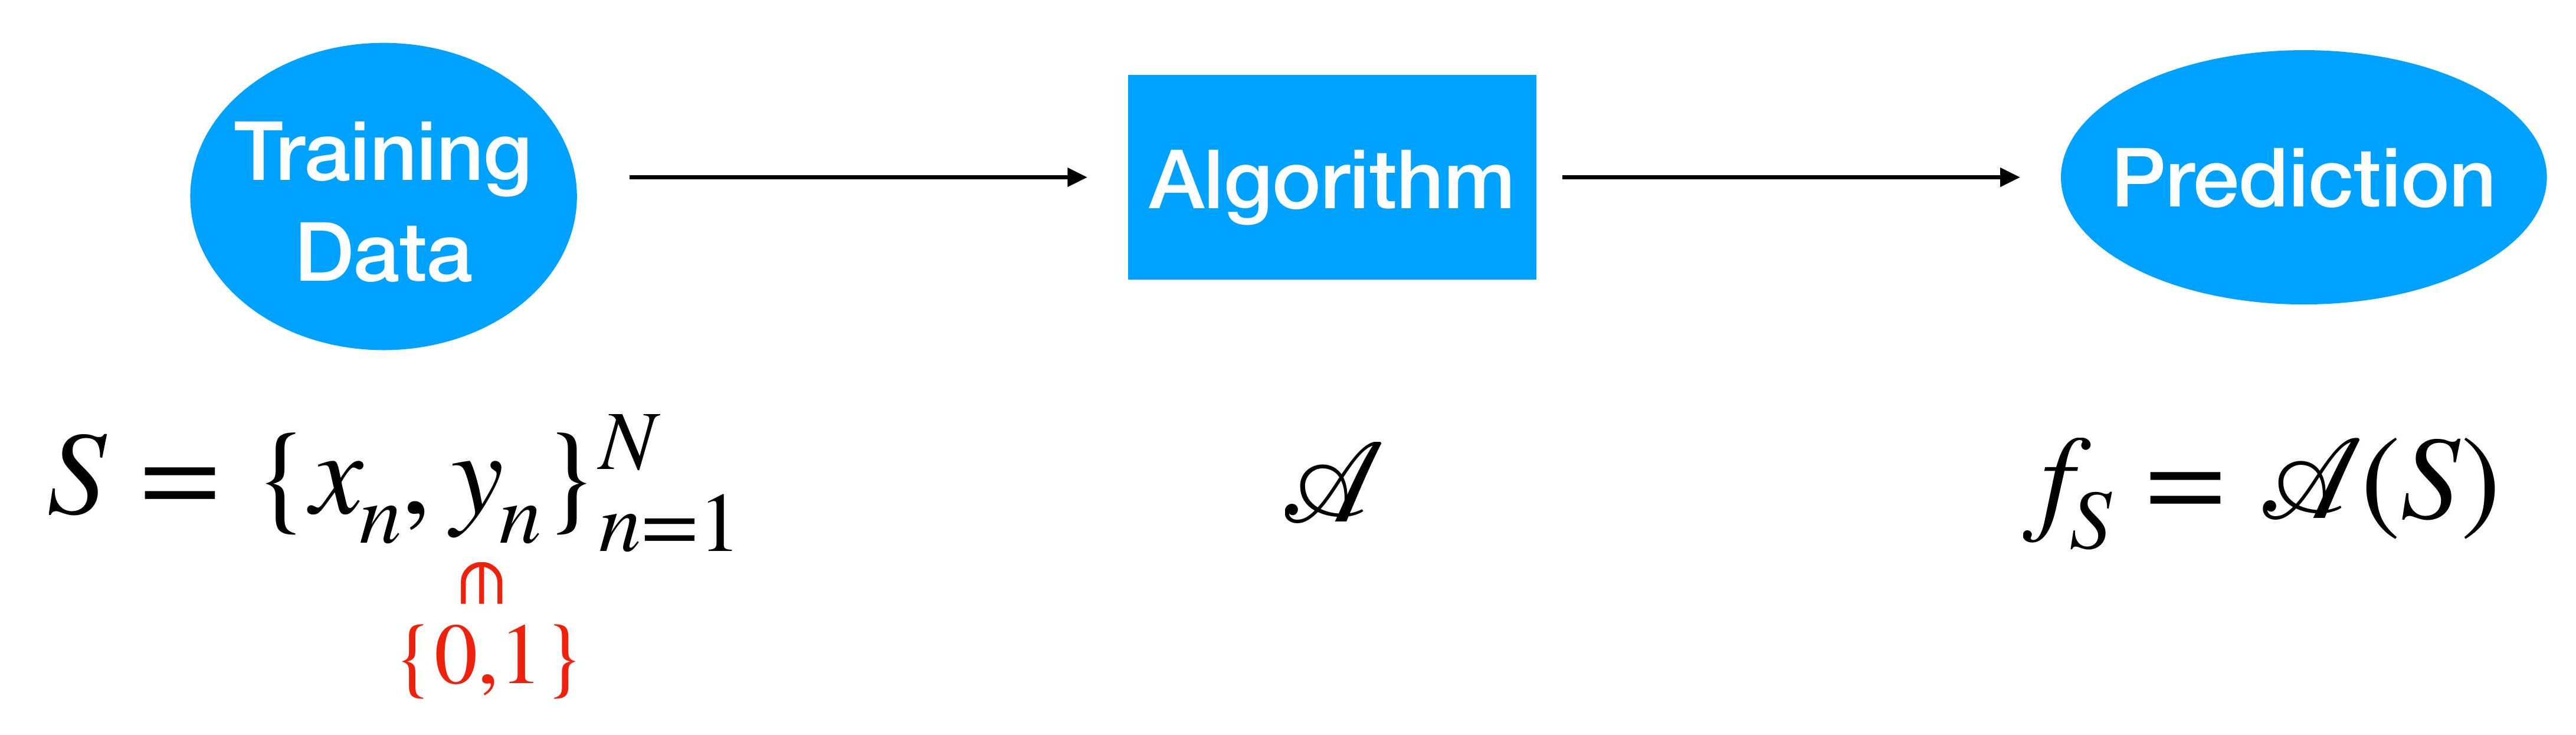
\includegraphics[max width=\textwidth]{2023_12_30_261a5c67f471a6c49904g-02}
\end{center}

\section*{Motivation for logistic regression}
Instead of directly modeling the output $Y$, we can model the probability that $Y$ belongs to a specific class. How?

In the previous lecture, we used a linear regression model $\mathbb{P}(Y=1 \mid X=x)=x^{\top} w+w_{0}$ but

\begin{itemize}
  \item The predicted value is not in $[0,1]$
  \item Very large or small prediction values contribute to the error even when they suggest high confidence in the resulting classification
\end{itemize}

\begin{center}
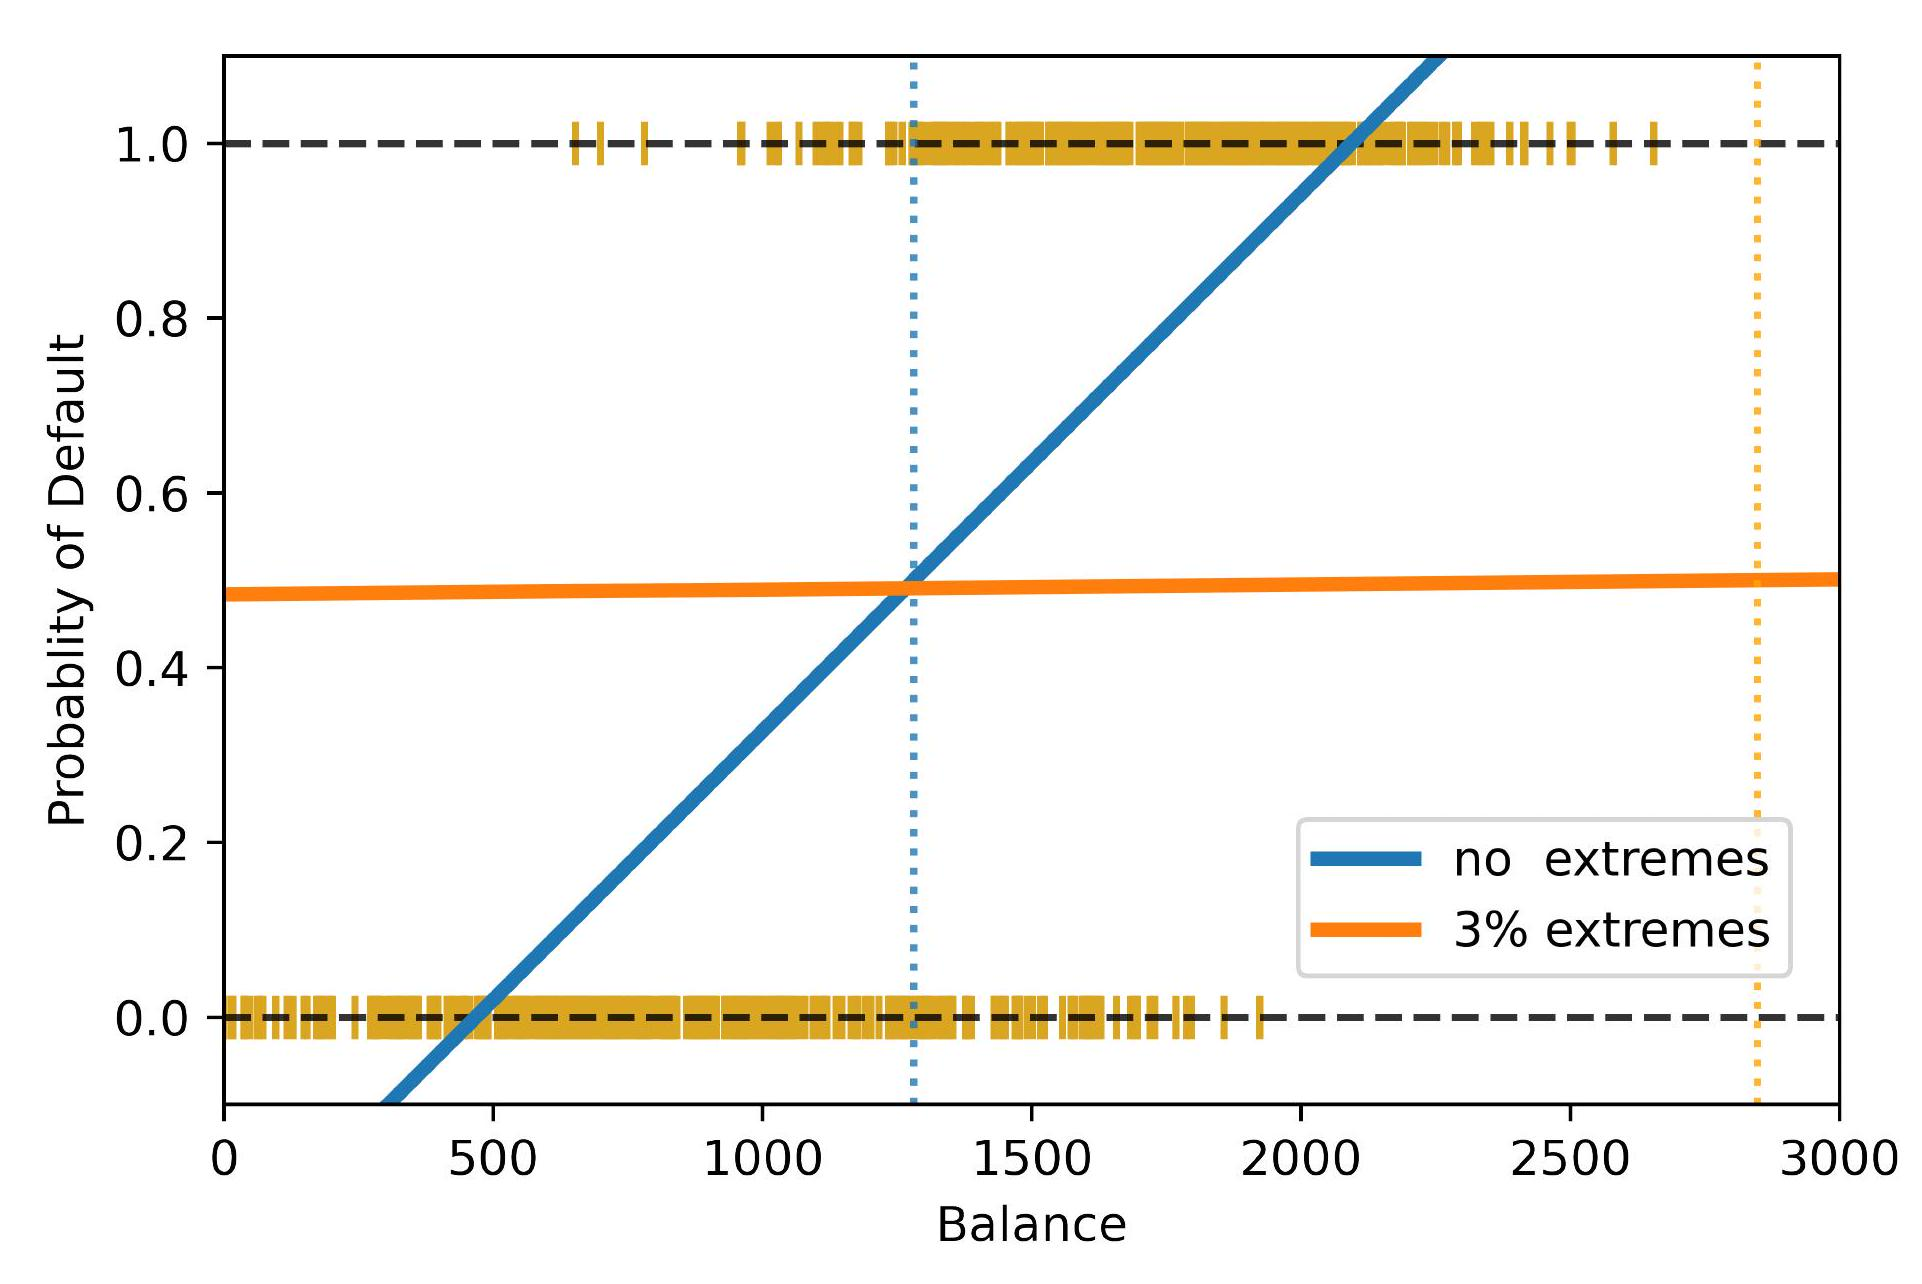
\includegraphics[max width=\textwidth]{2023_12_30_261a5c67f471a6c49904g-03}
\end{center}

Solution: map the prediction from $(-\infty,+\infty)$ to $[0,1]$

\section*{The logistic function}
$$
\sigma(\eta):=\frac{e^{\eta}}{1+e^{\eta}}
$$

Properties of the logistic function:

\begin{center}
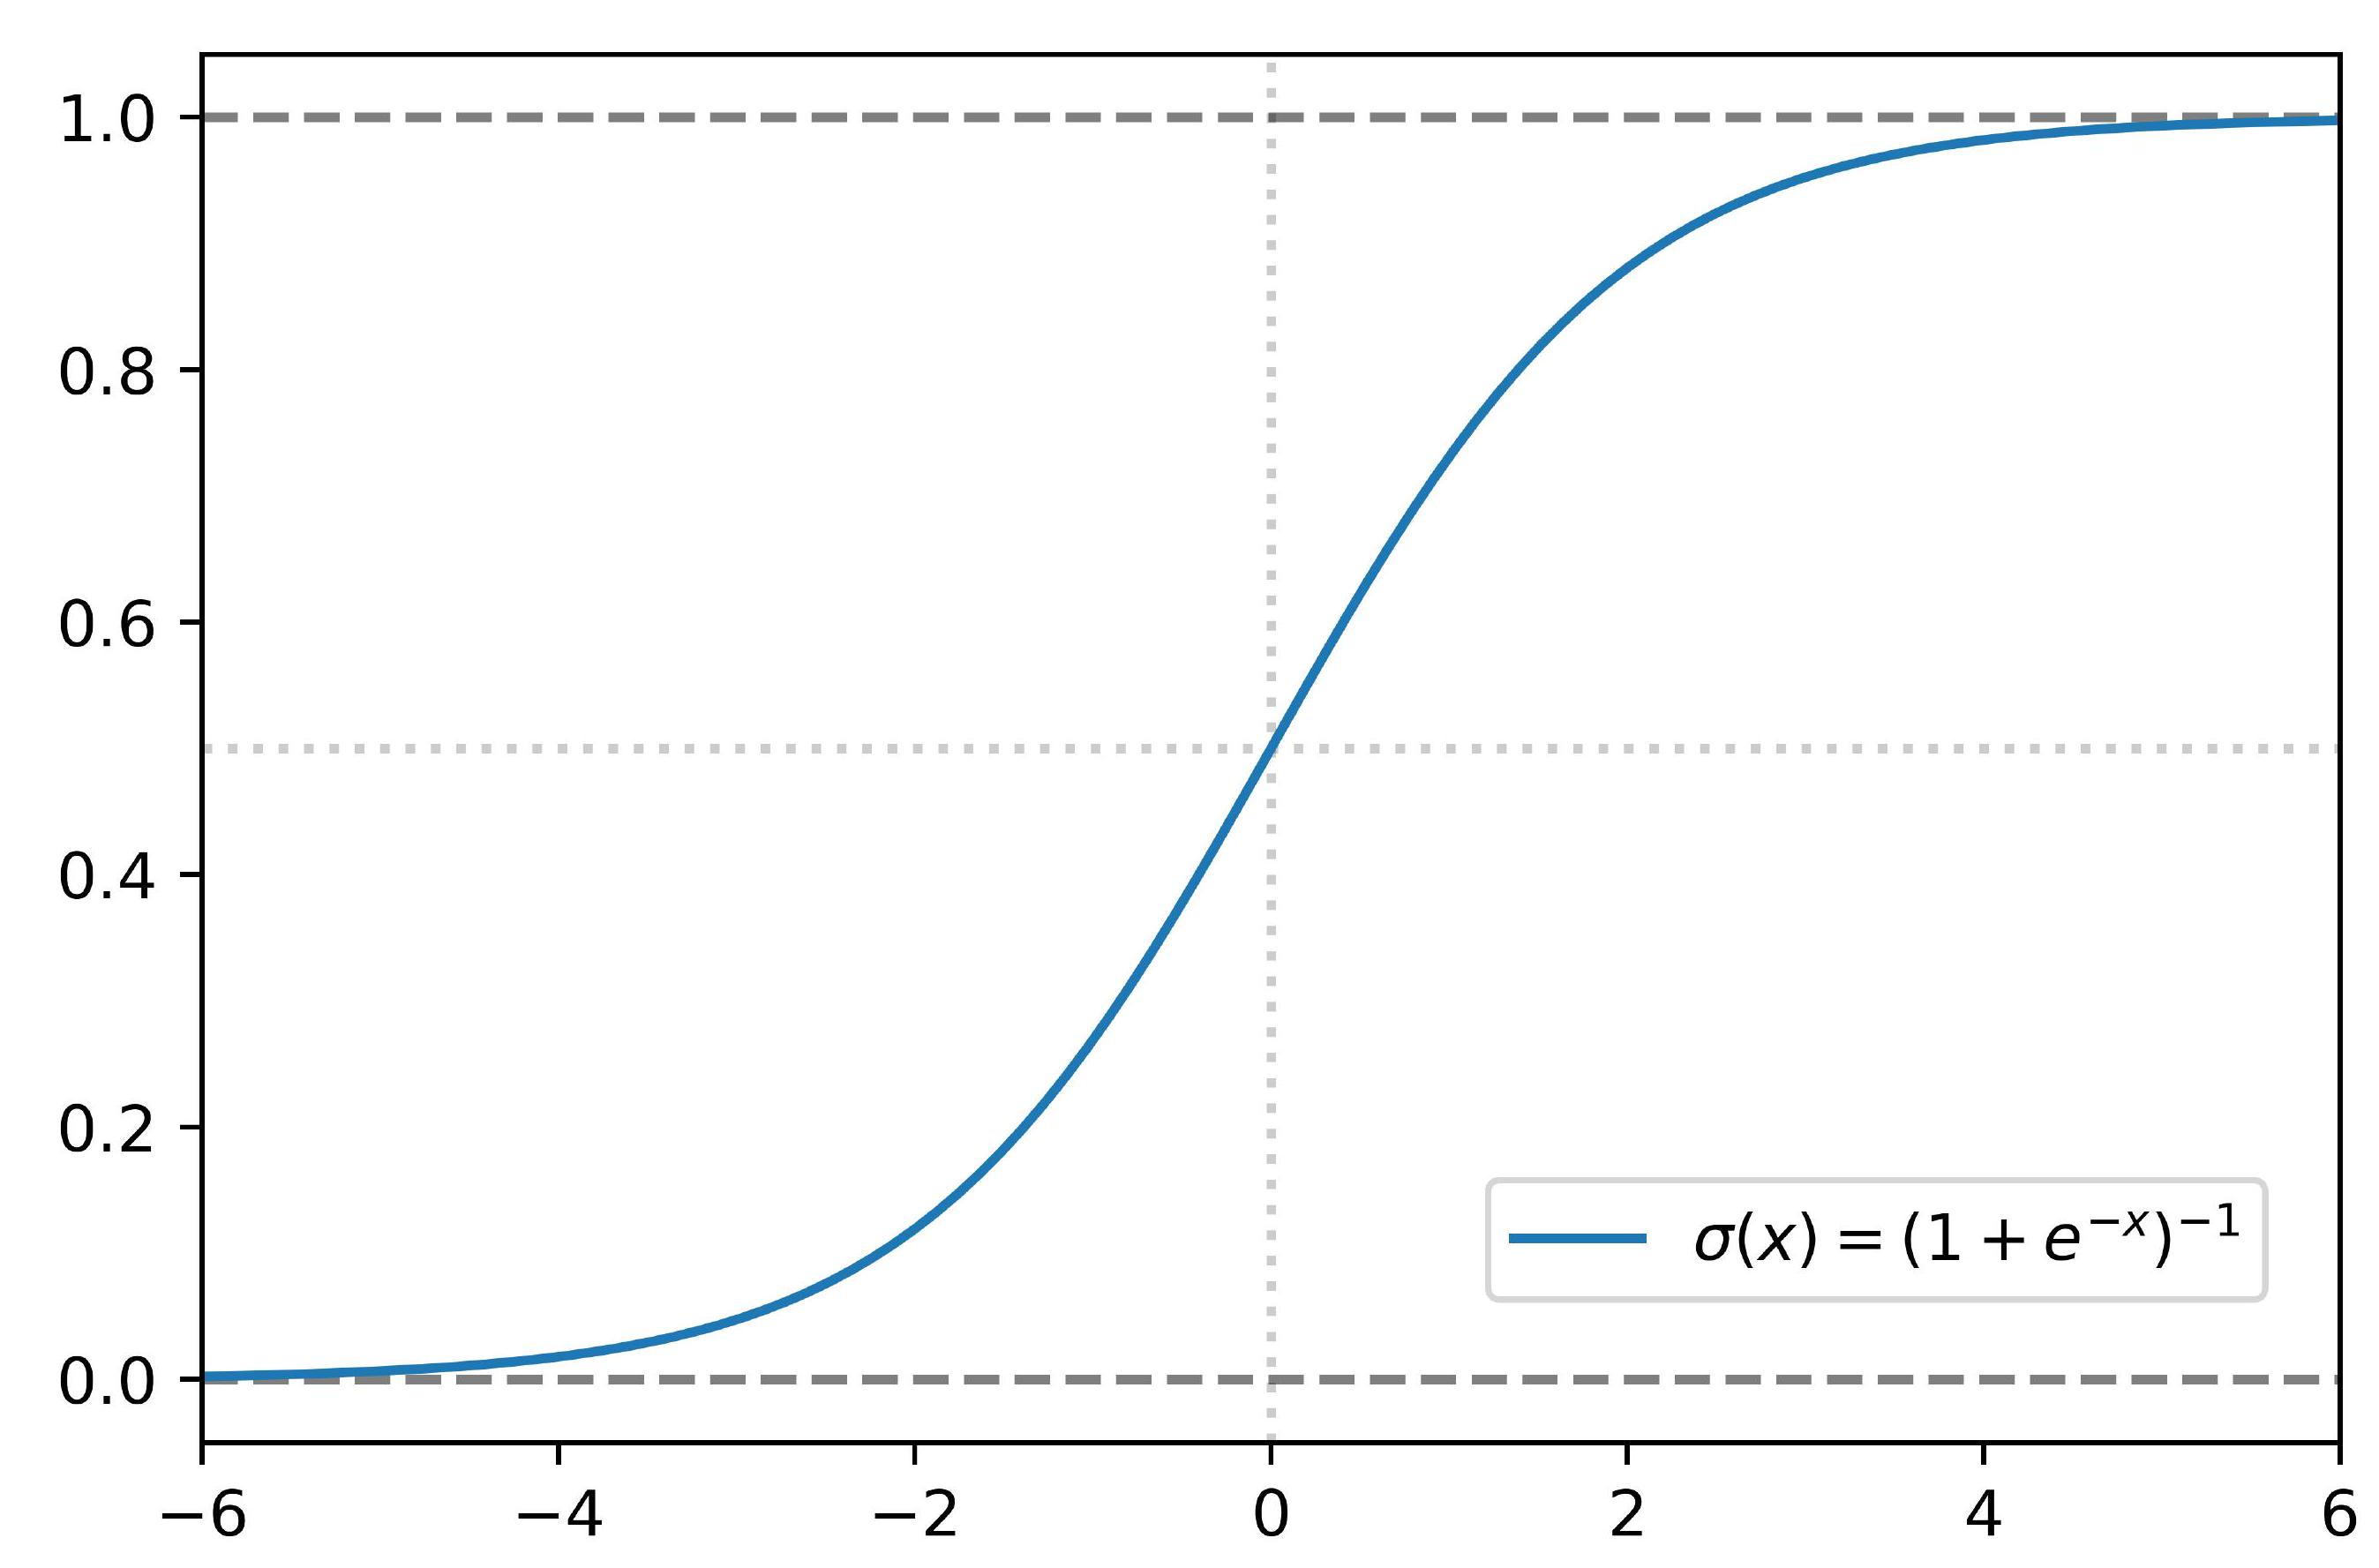
\includegraphics[max width=\textwidth]{2023_12_30_261a5c67f471a6c49904g-04}
\end{center}

$1-\sigma(\eta)=\frac{1+e^{\eta}-e^{\eta}}{1+e^{\eta}}=\left(1+e^{\eta}\right)^{-1}$
$\sigma^{\prime}(\eta)=\frac{e^{\eta}\left(1+e^{\eta}\right)-e^{\eta} e^{\eta}}{\left(1+e^{\eta}\right)^{2}}=\frac{e^{\eta}}{\left(1+e^{\eta}\right)^{2}}=\sigma(\eta)(1-\sigma(\eta))$

\section*{Logistic Regression}
$$
\begin{aligned}
& p(1 \mid x):=\mathbb{P}(Y=1 \mid X=x)=\sigma\left(x^{\top} w+w_{0}\right) \\
& p(0 \mid x):=\mathbb{P}(Y=0 \mid X=x)=1-\sigma\left(x^{\top} w+w_{0}\right)
\end{aligned}
$$

Logistic regression models the probability that $Y$ belongs to a particular class using the logistic function $\sigma$

Label prediction: quantize the probability:

$$
\begin{aligned}
& \text { If } p(1 \mid x) \geq 1 / 2, \text { you predict the class } 1 \\
& \text { If } p(1 \mid x)<1 / 2 \text {, you predict the class } 0
\end{aligned}
$$

Interpretation:

\begin{itemize}
  \item Very large $\left|x^{\top} w+w_{0}\right|$ corresponds to $p(1 \mid x)$ very close to 0 or 1 (high confidence)
  \item Small $\left|x^{\top} w+w_{0}\right|$ corresponds to $p(1 \mid x)$ very close to .5 (low confidence)
\end{itemize}

\section*{Comparison of logistic and linear regression for balanced data}
\begin{center}
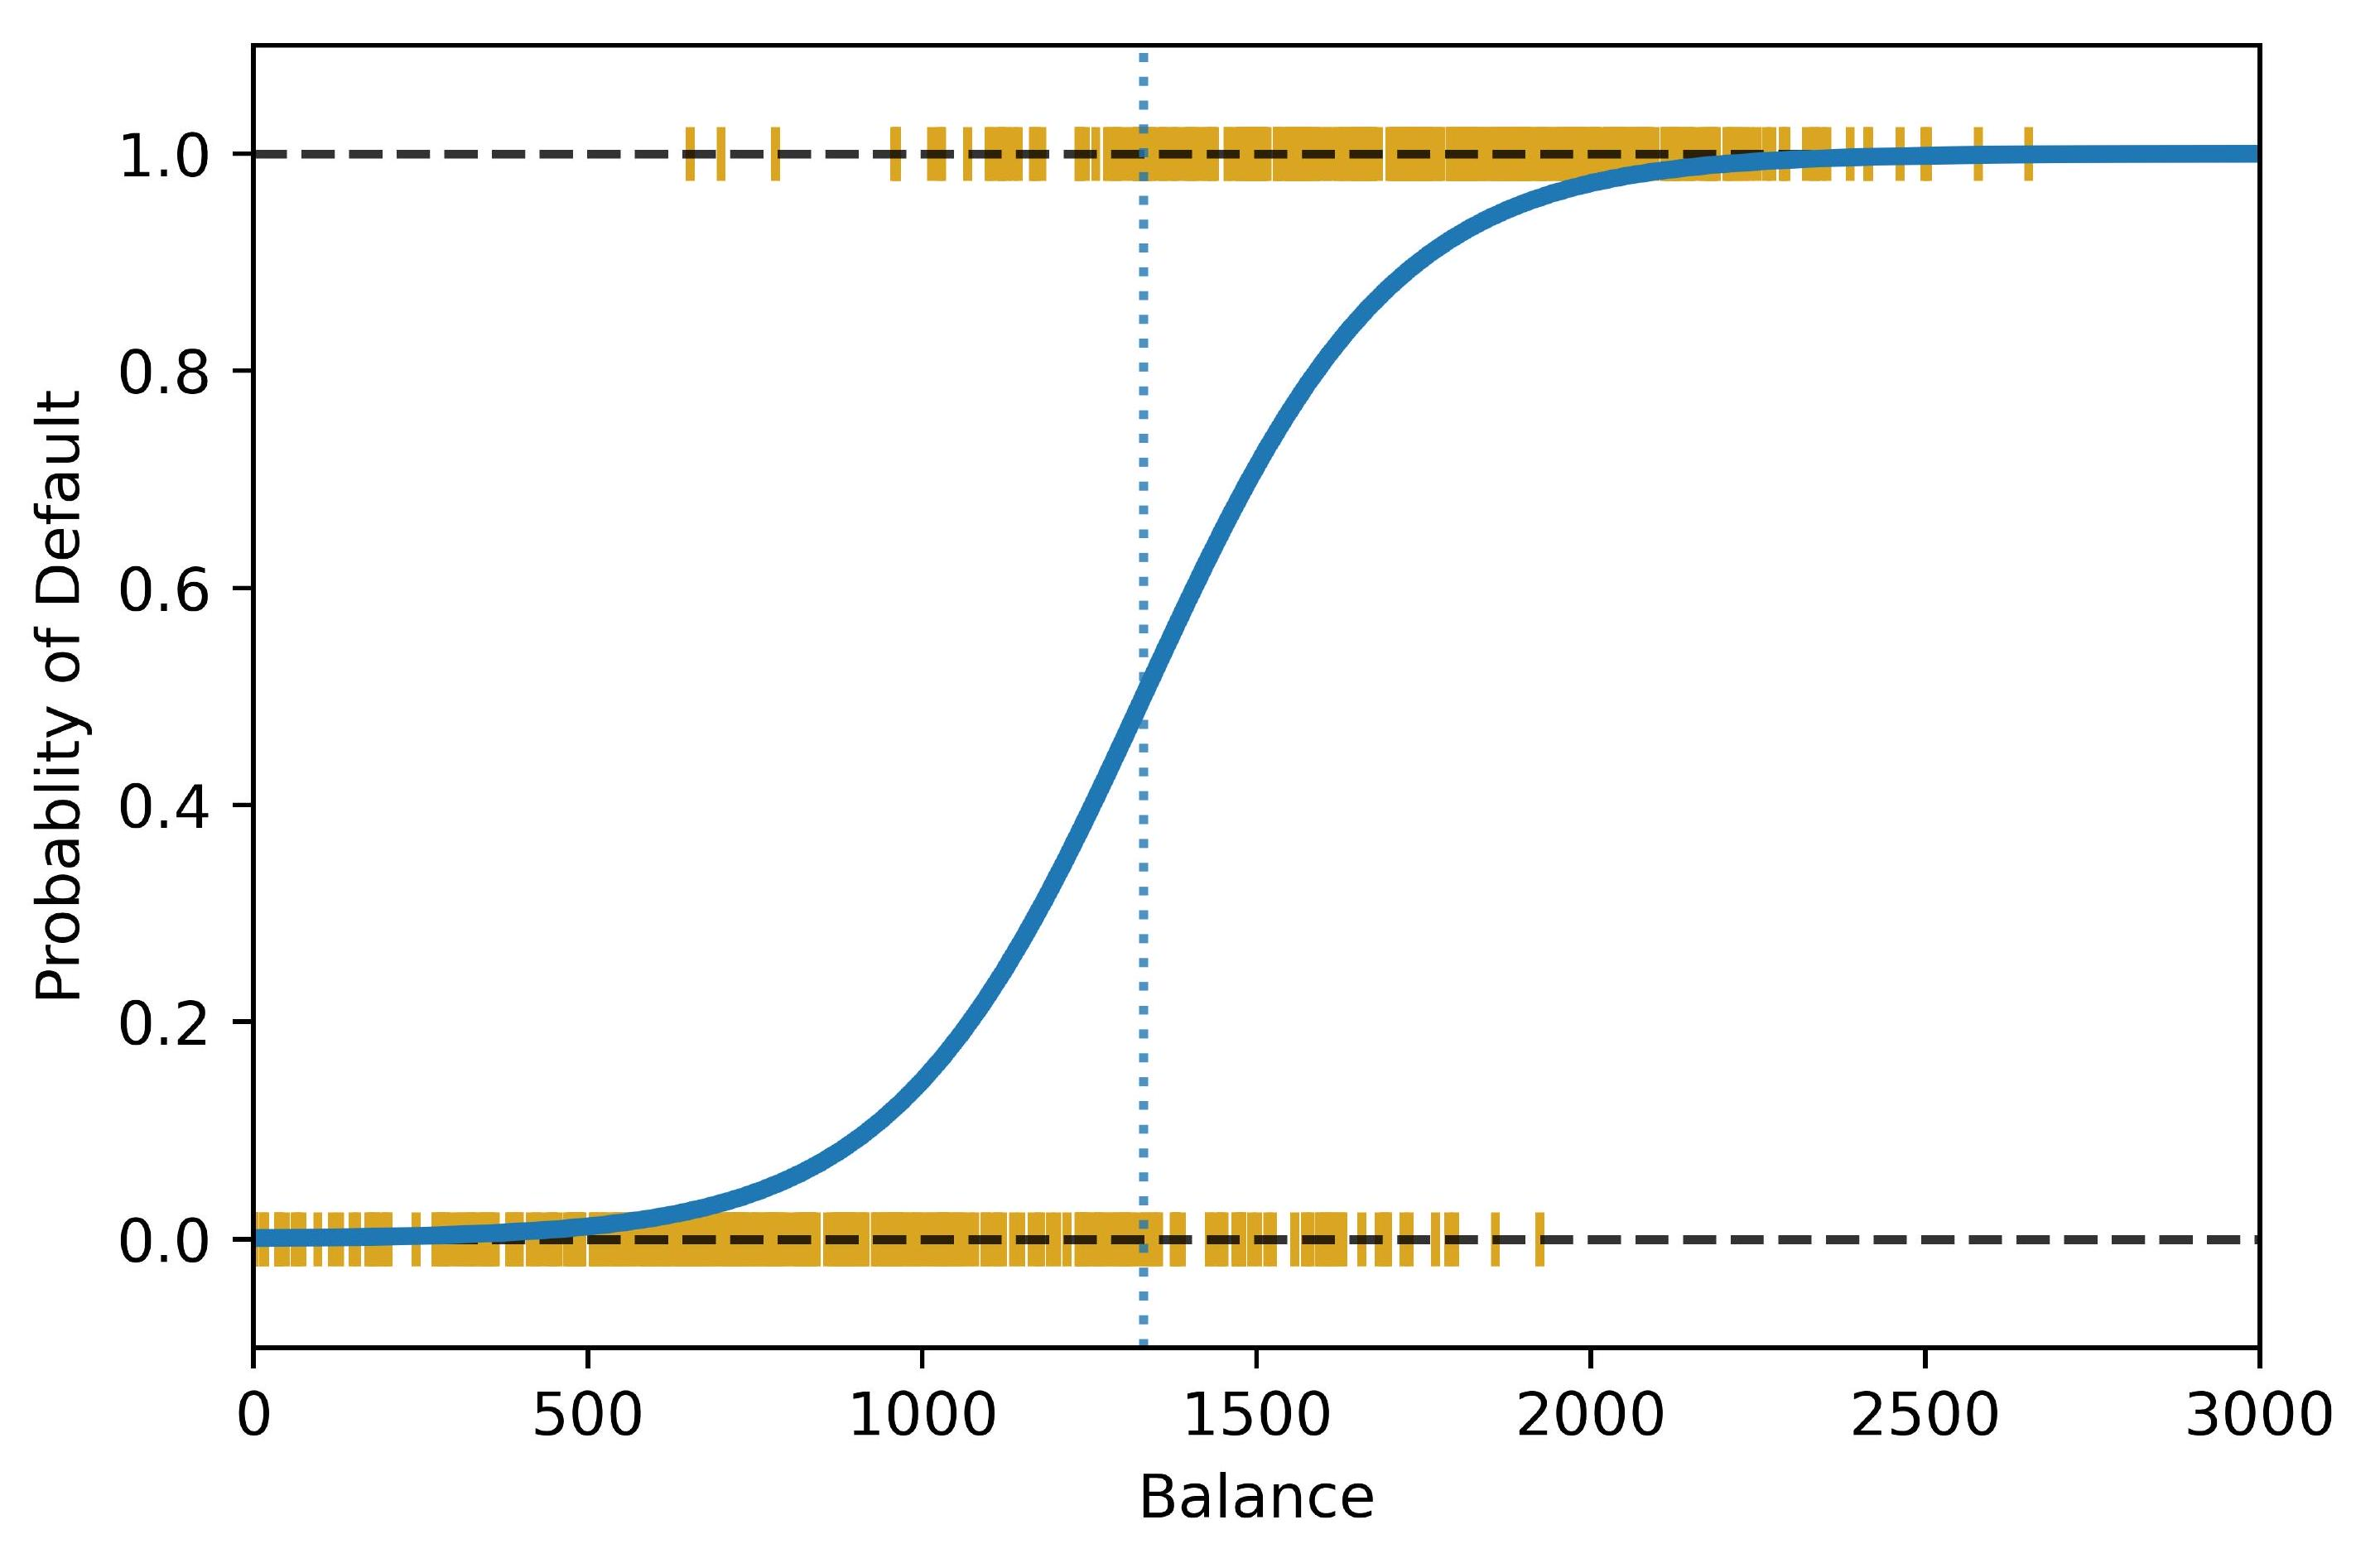
\includegraphics[max width=\textwidth]{2023_12_30_261a5c67f471a6c49904g-06(1)}
\end{center}

Logistic regression

\begin{center}
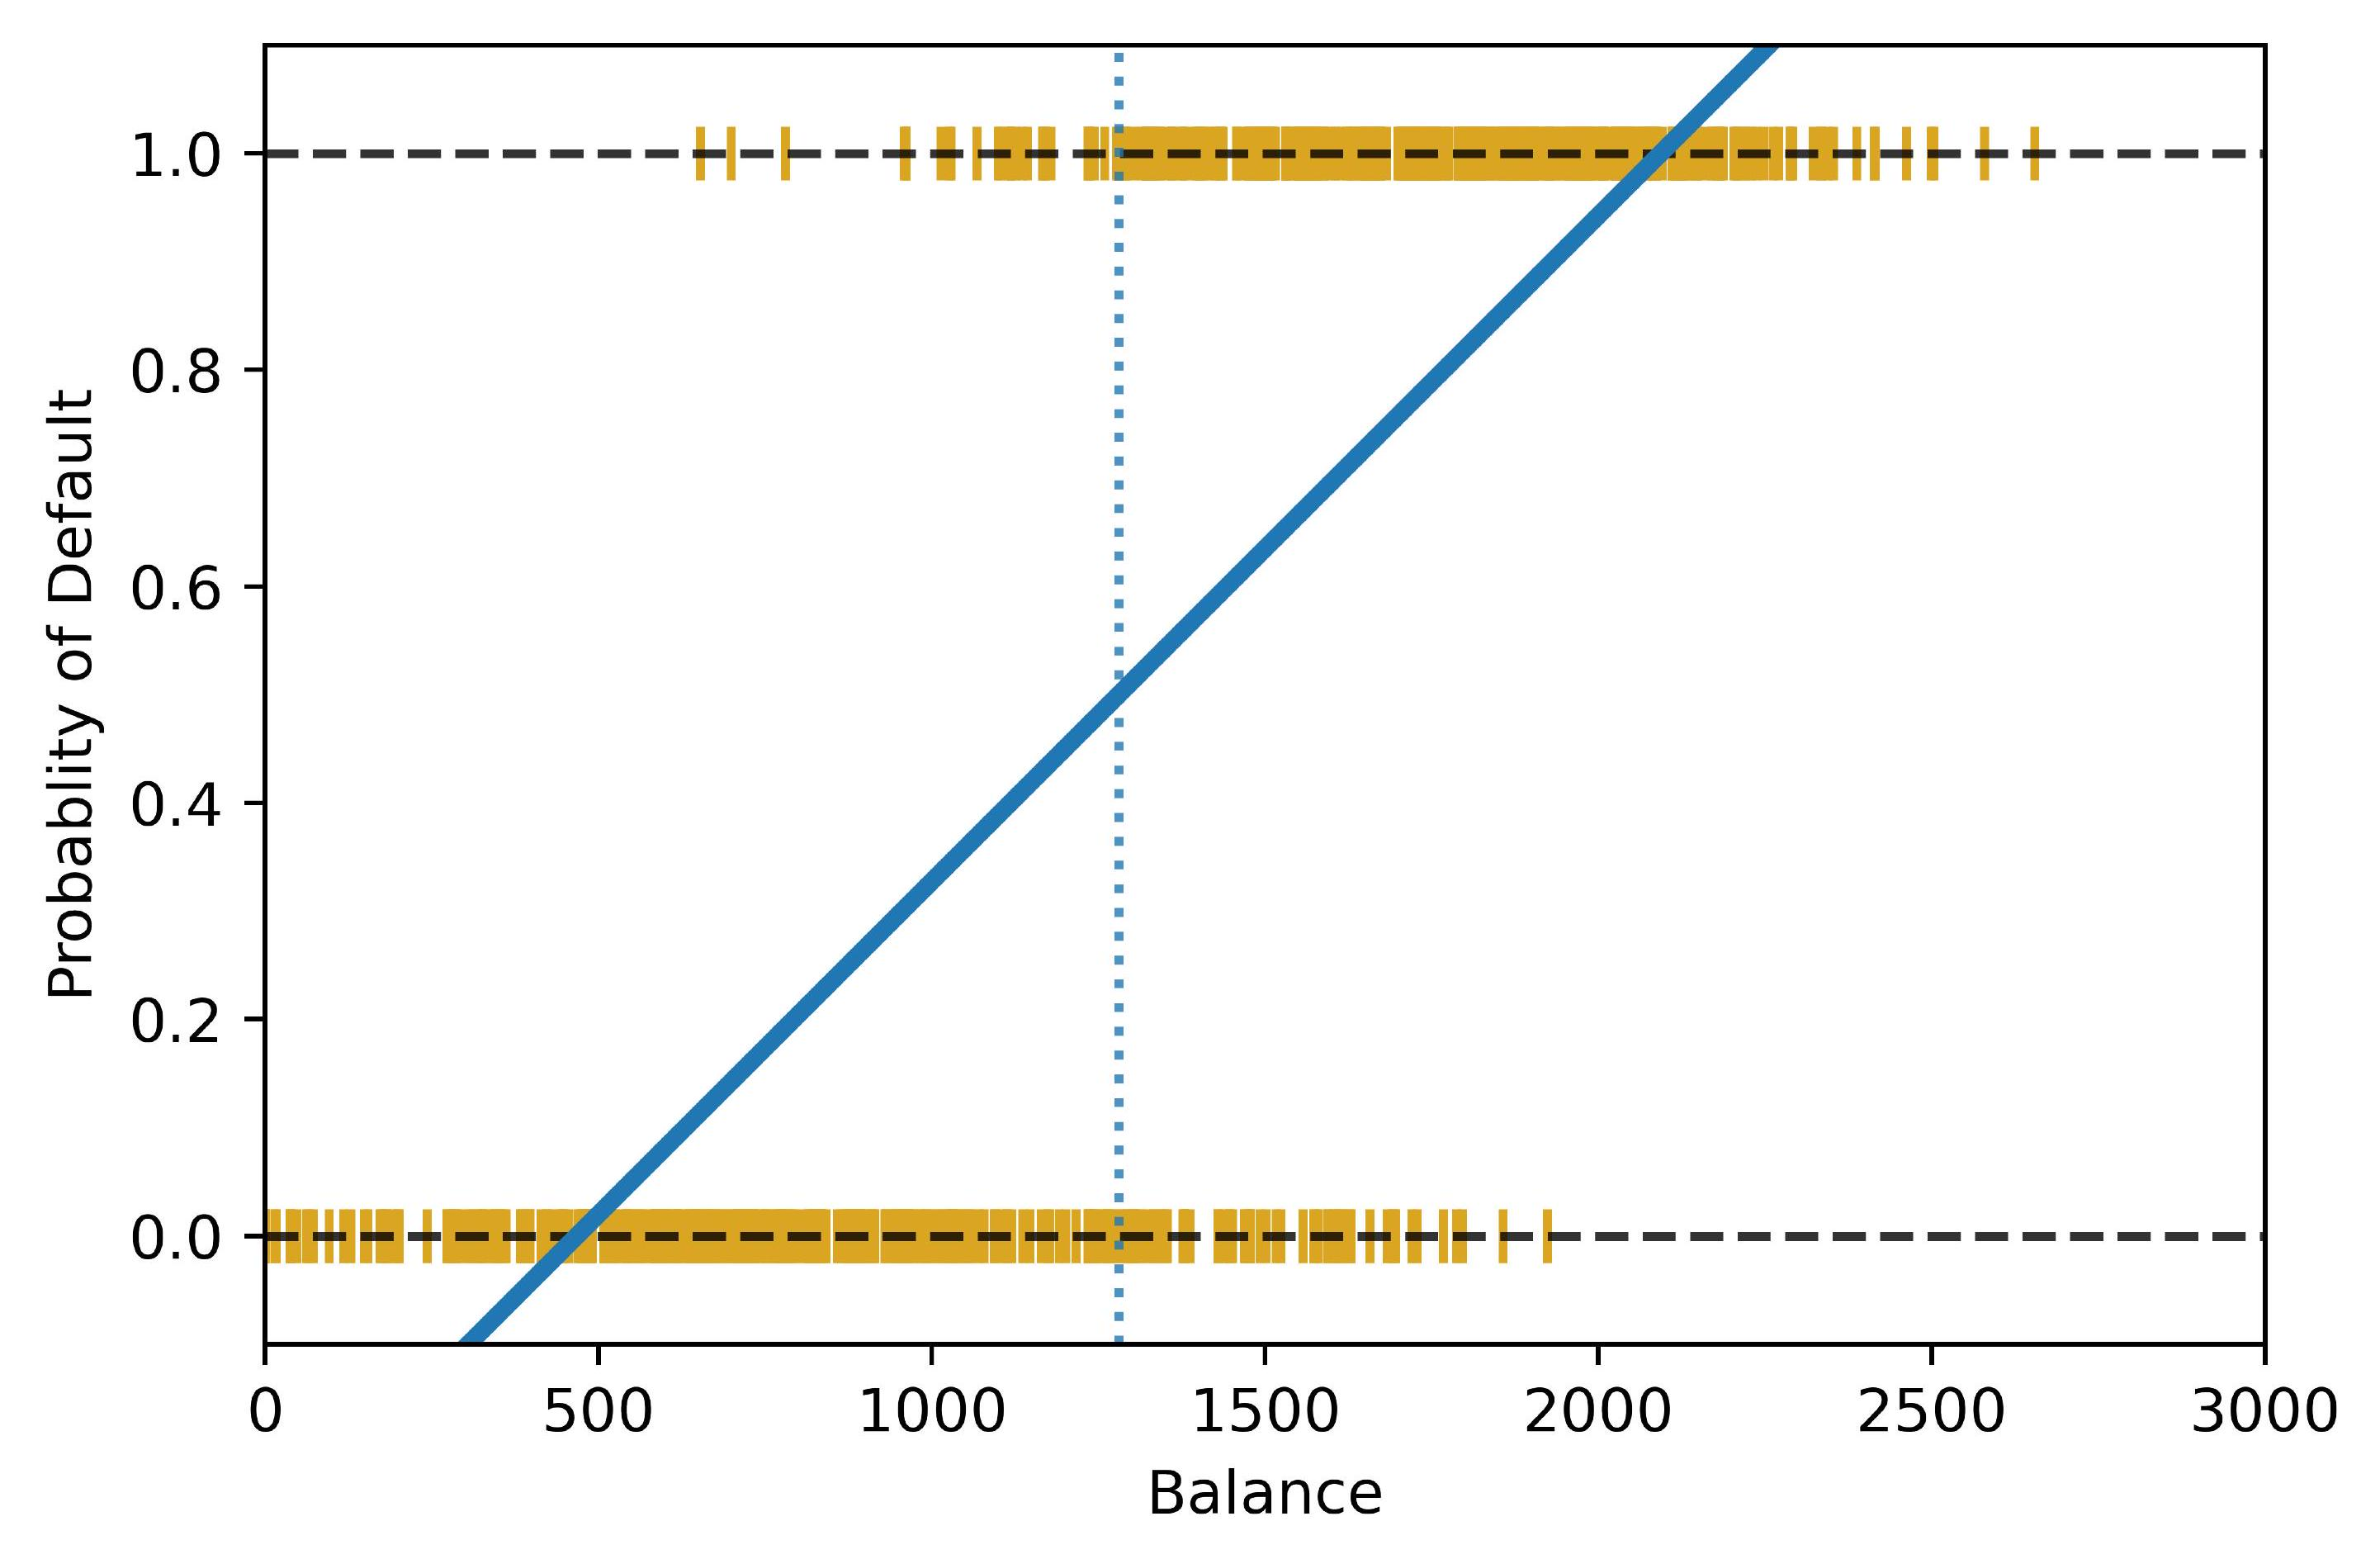
\includegraphics[max width=\textwidth]{2023_12_30_261a5c67f471a6c49904g-06}
\end{center}

Linear regression

\section*{Comparison of logistic and linear regression for unbalanced data}
\begin{center}
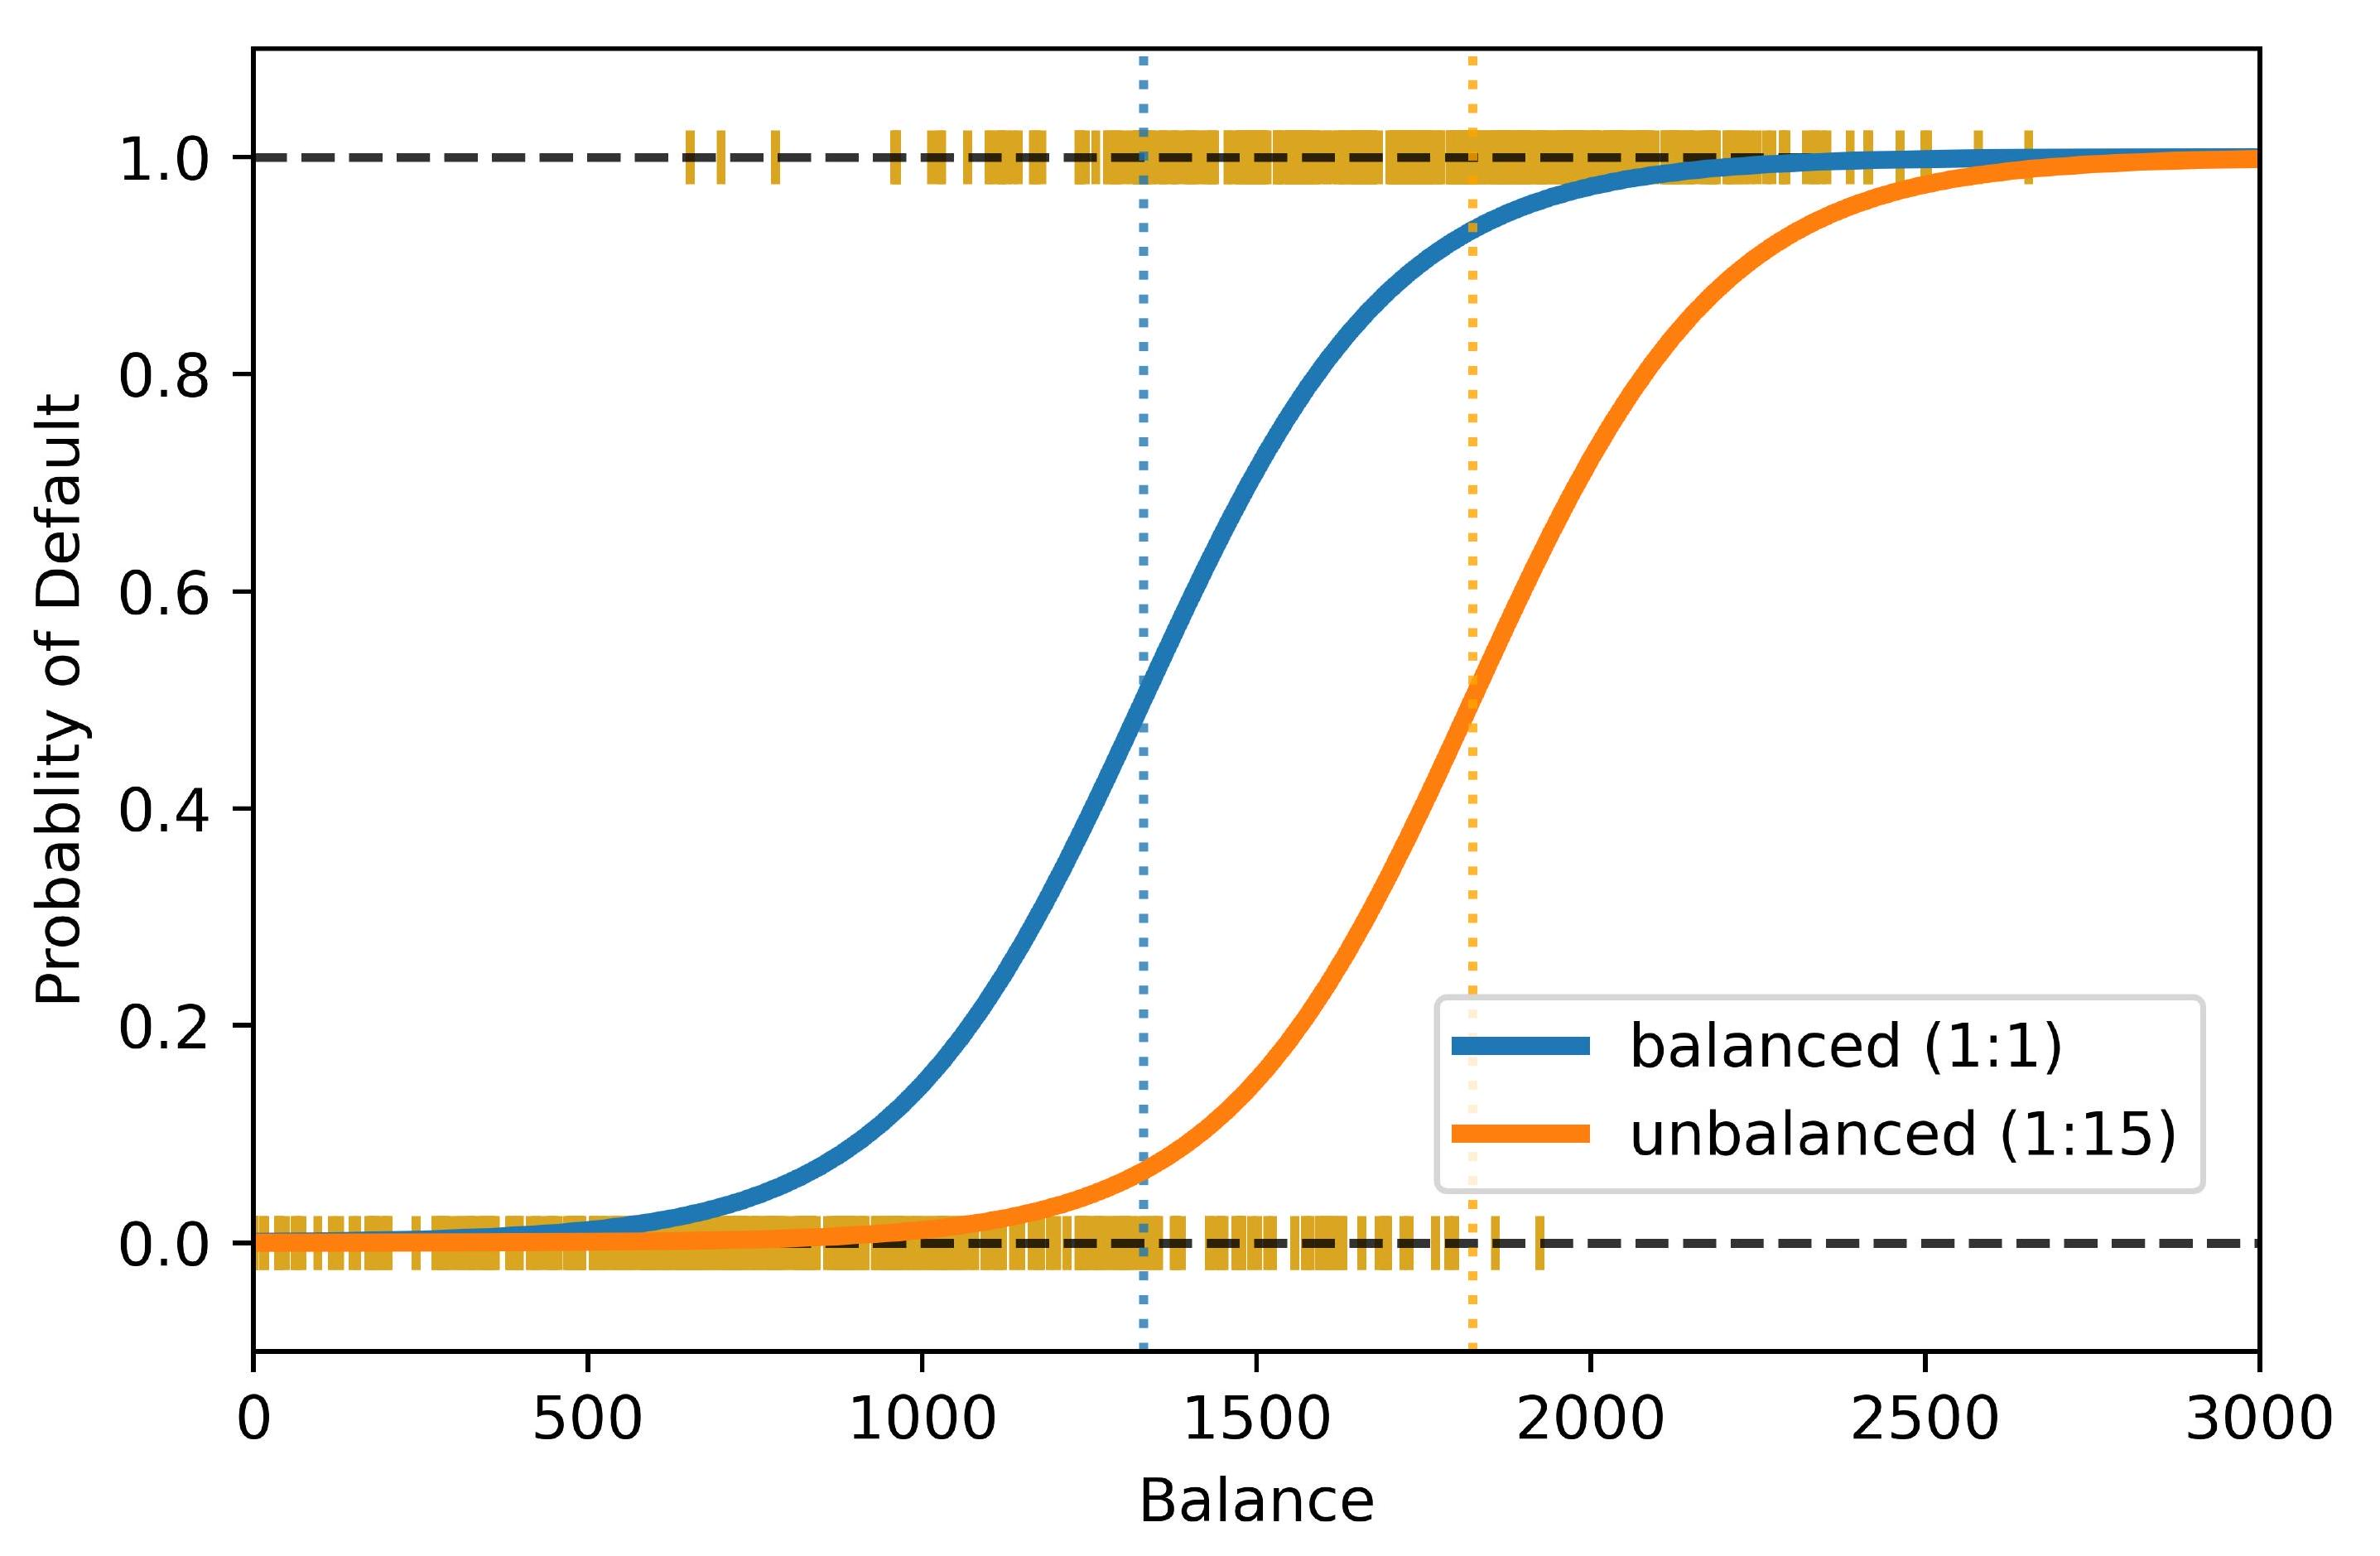
\includegraphics[max width=\textwidth]{2023_12_30_261a5c67f471a6c49904g-07(1)}
\end{center}

Logistic regression

\begin{center}
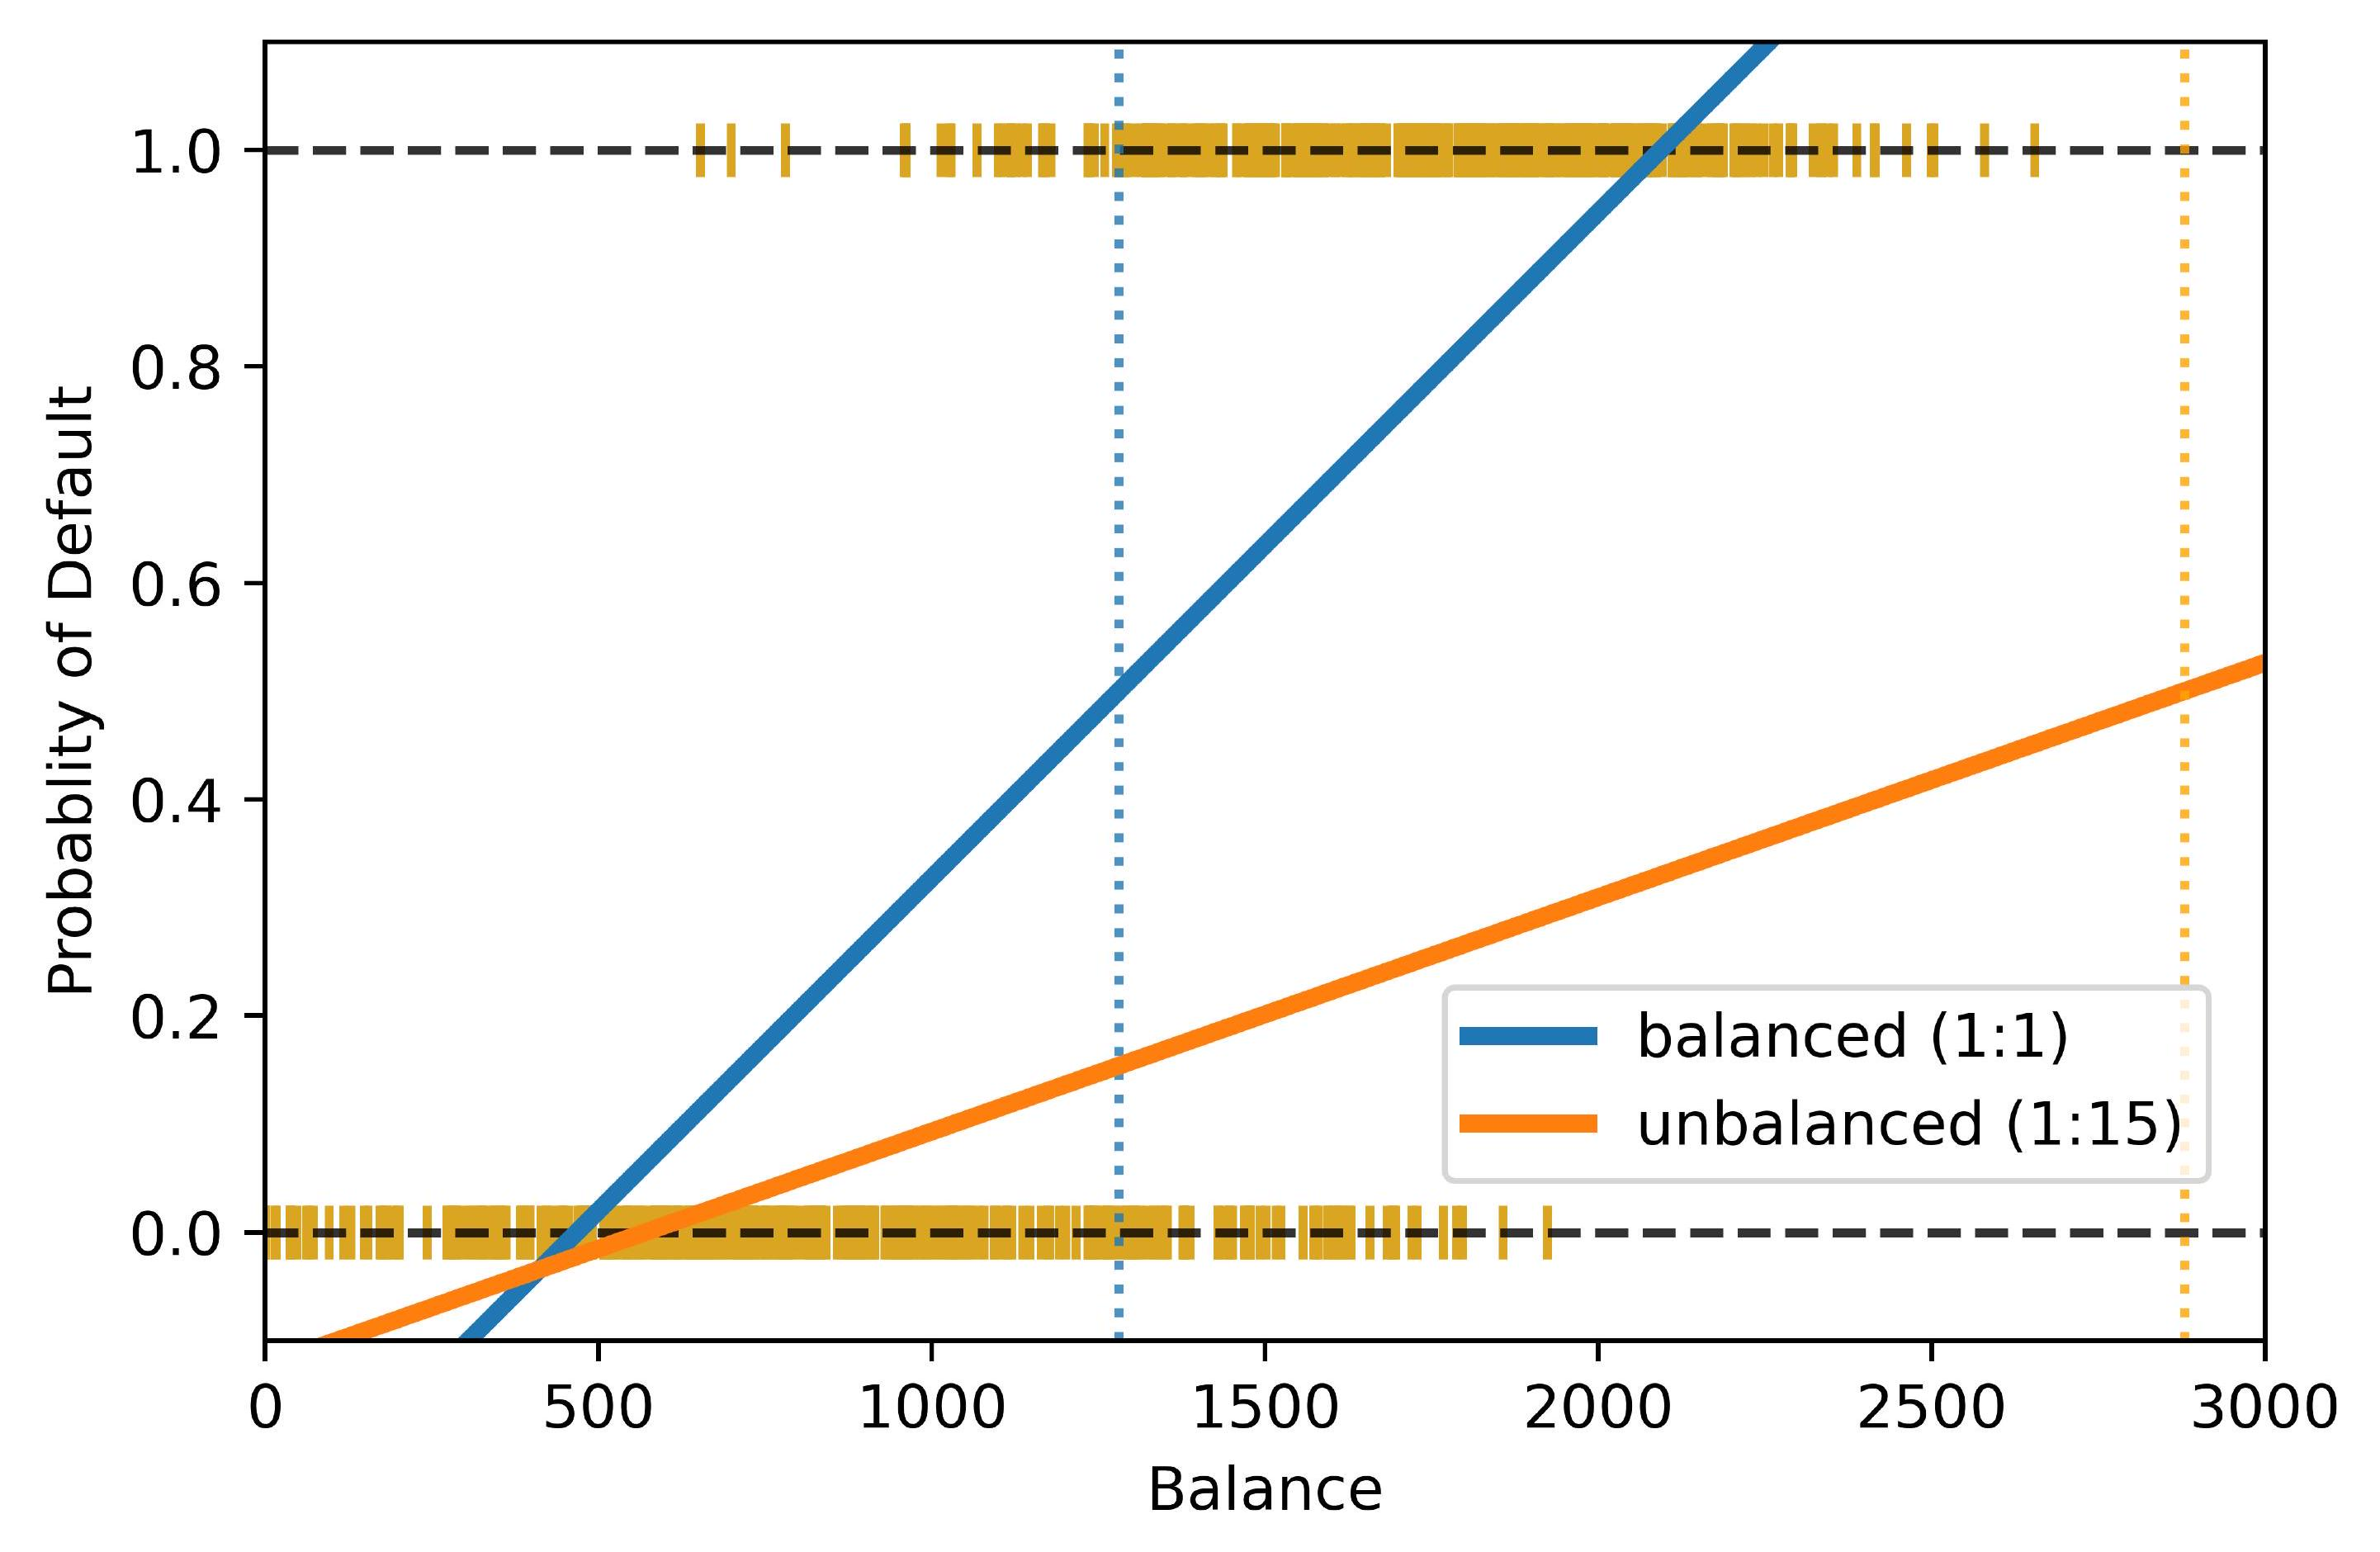
\includegraphics[max width=\textwidth]{2023_12_30_261a5c67f471a6c49904g-07}
\end{center}

Linear regression

\section*{Comparison of logistic and linear regression for data with extreme values}
\begin{center}
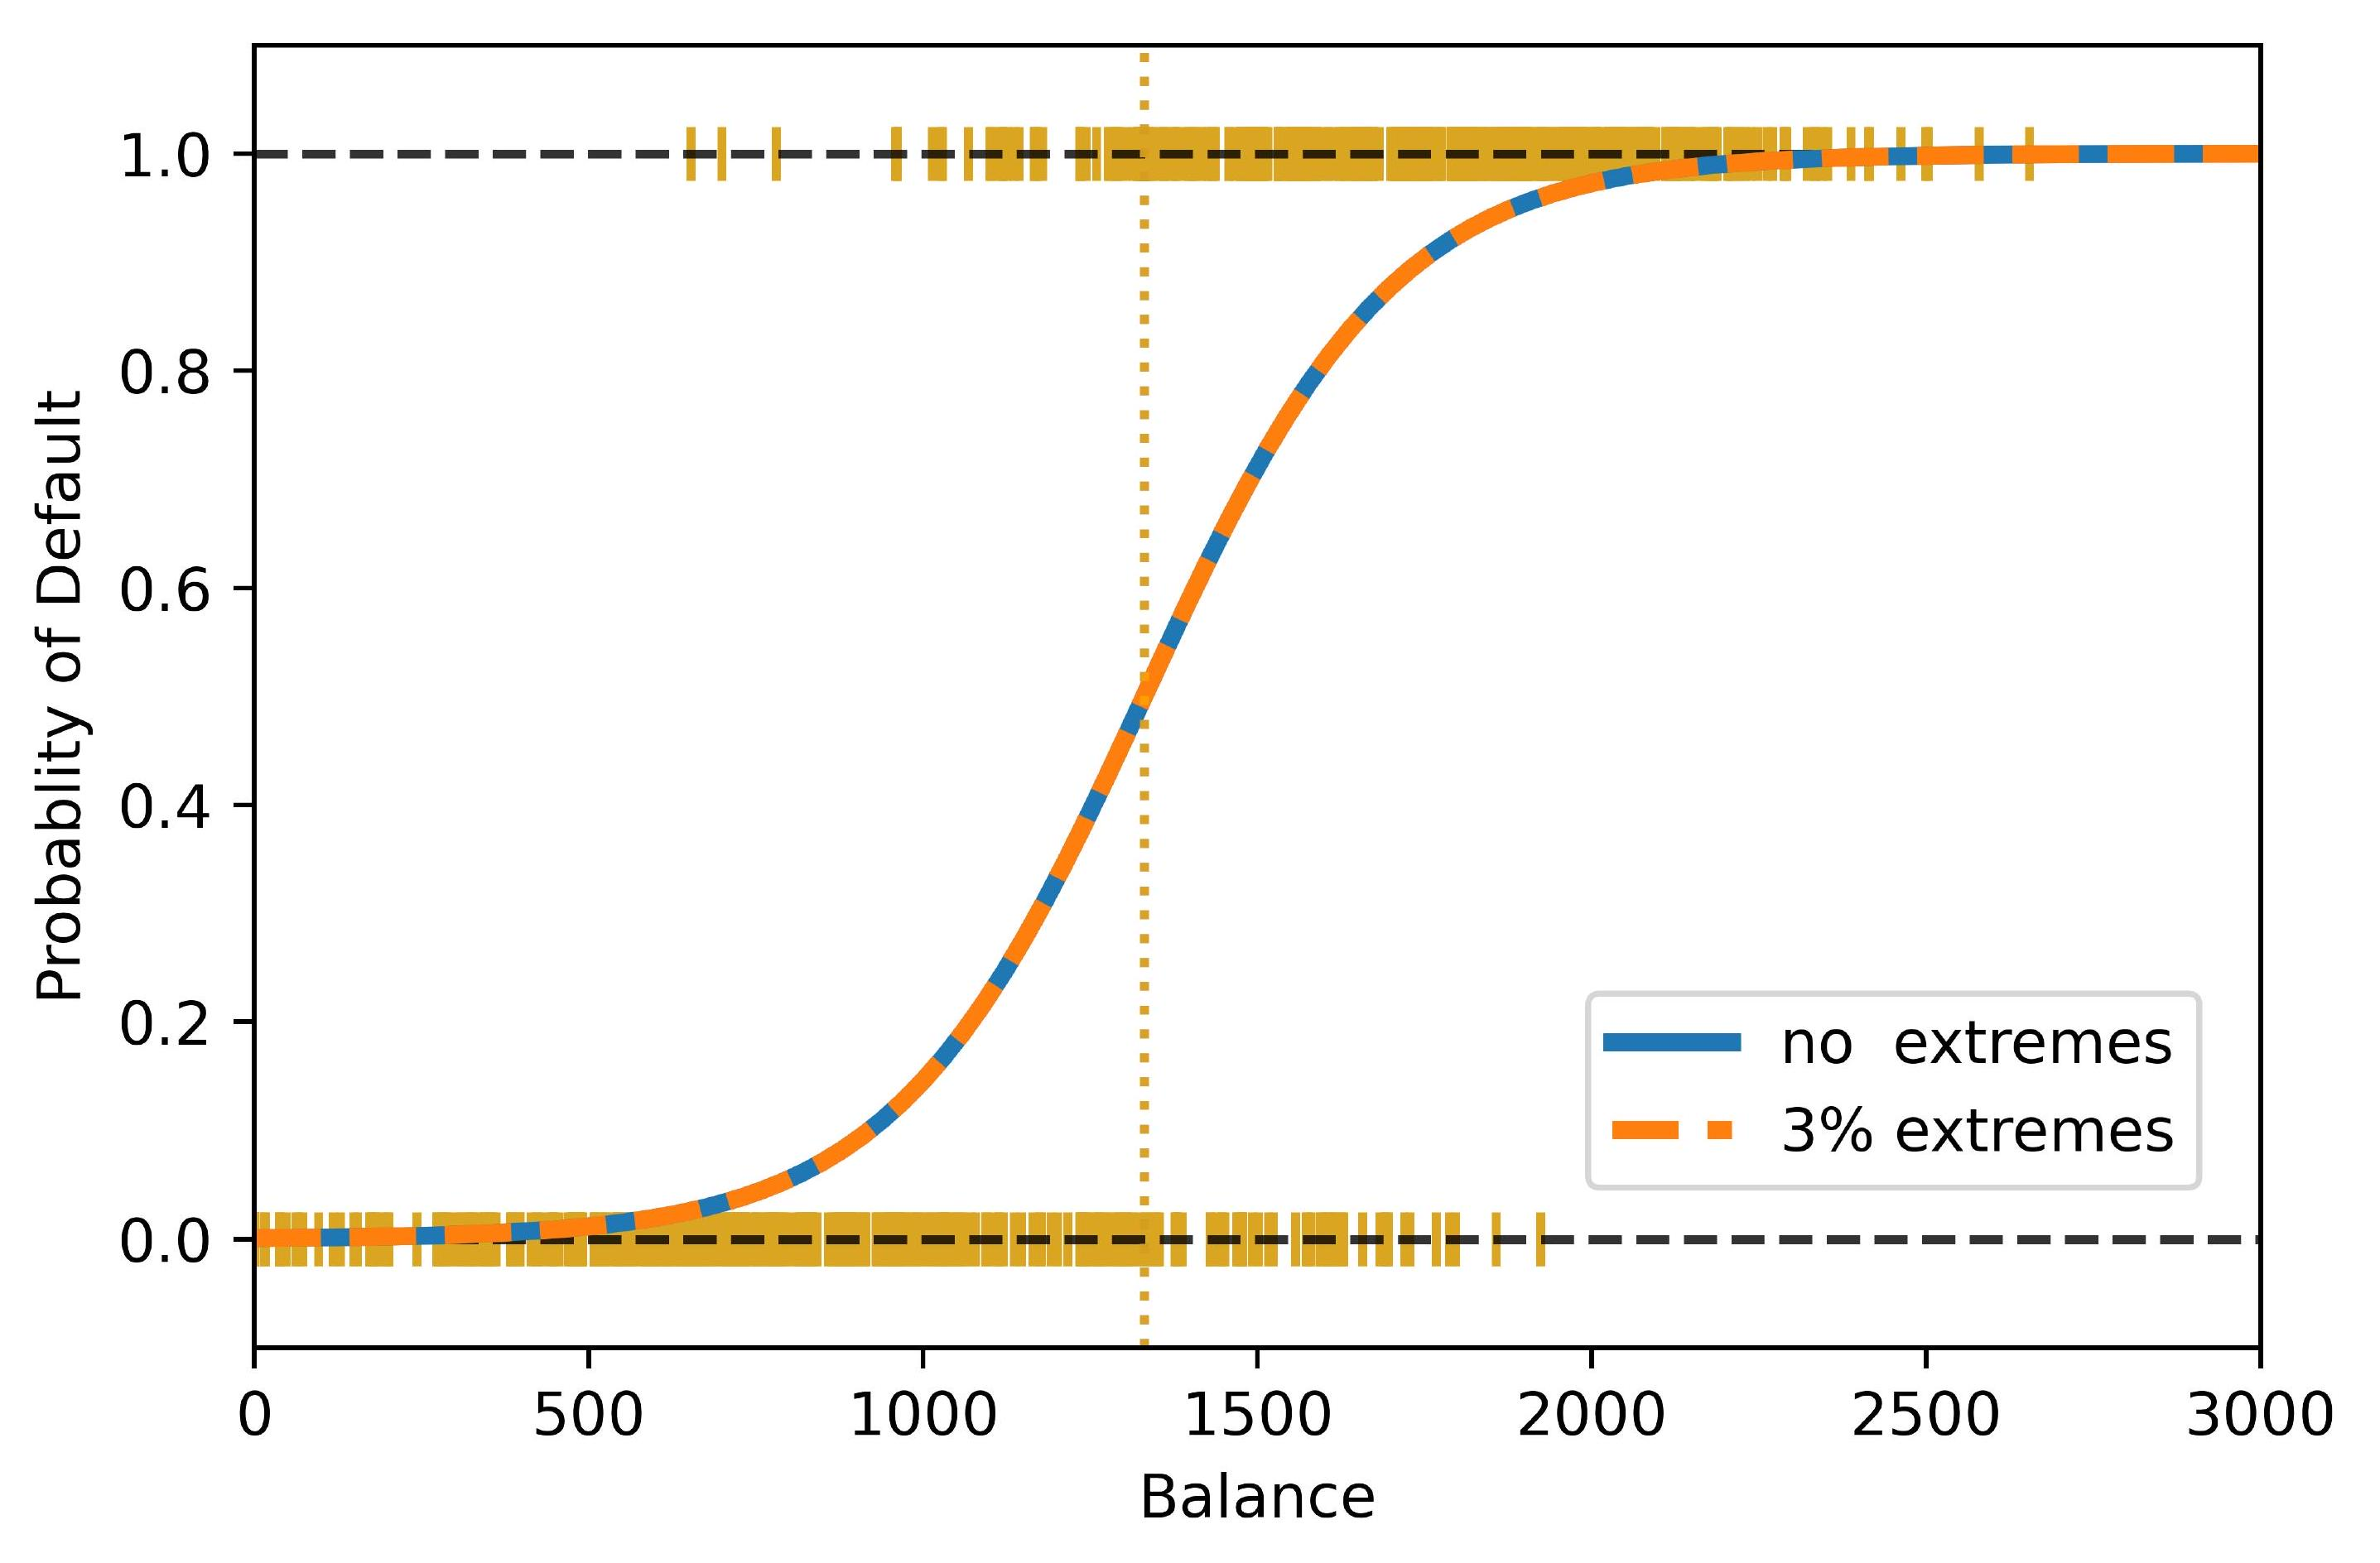
\includegraphics[max width=\textwidth]{2023_12_30_261a5c67f471a6c49904g-08}
\end{center}

Logistic regression

\begin{center}
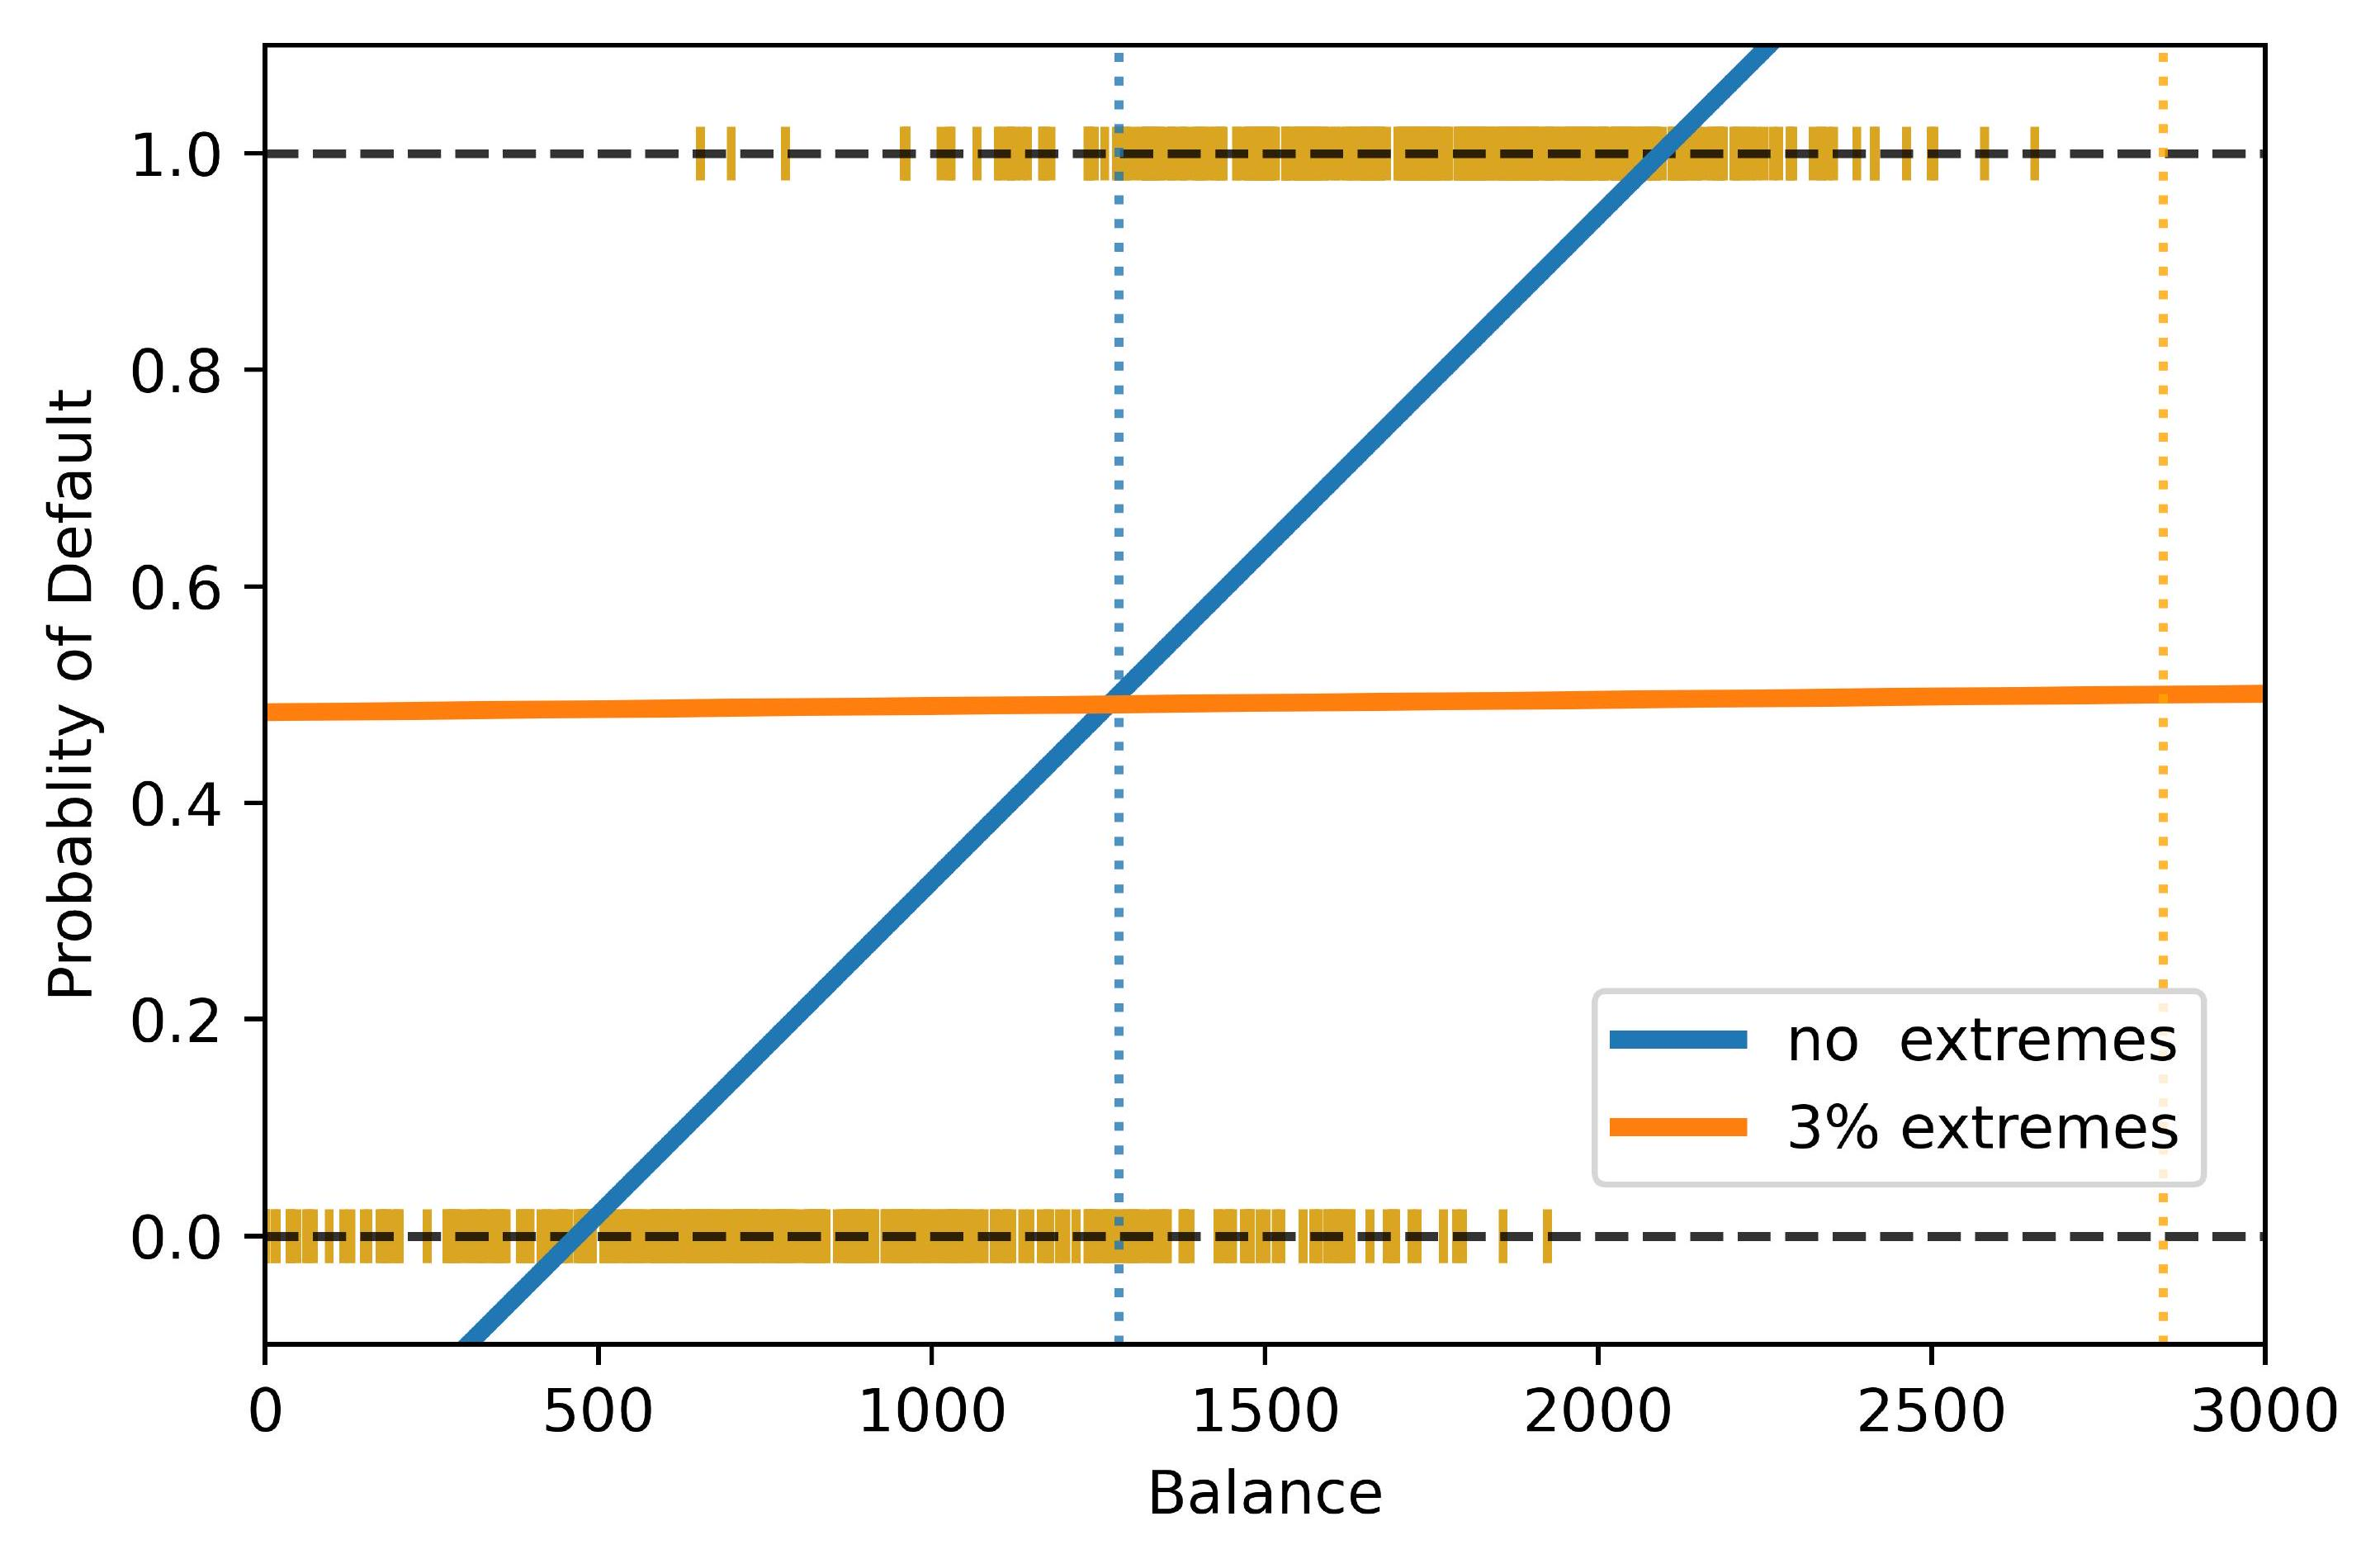
\includegraphics[max width=\textwidth]{2023_12_30_261a5c67f471a6c49904g-08(1)}
\end{center}

Linear regression

\section*{The vector $w$ is orthogonal to the "surface of transition"}
\begin{center}
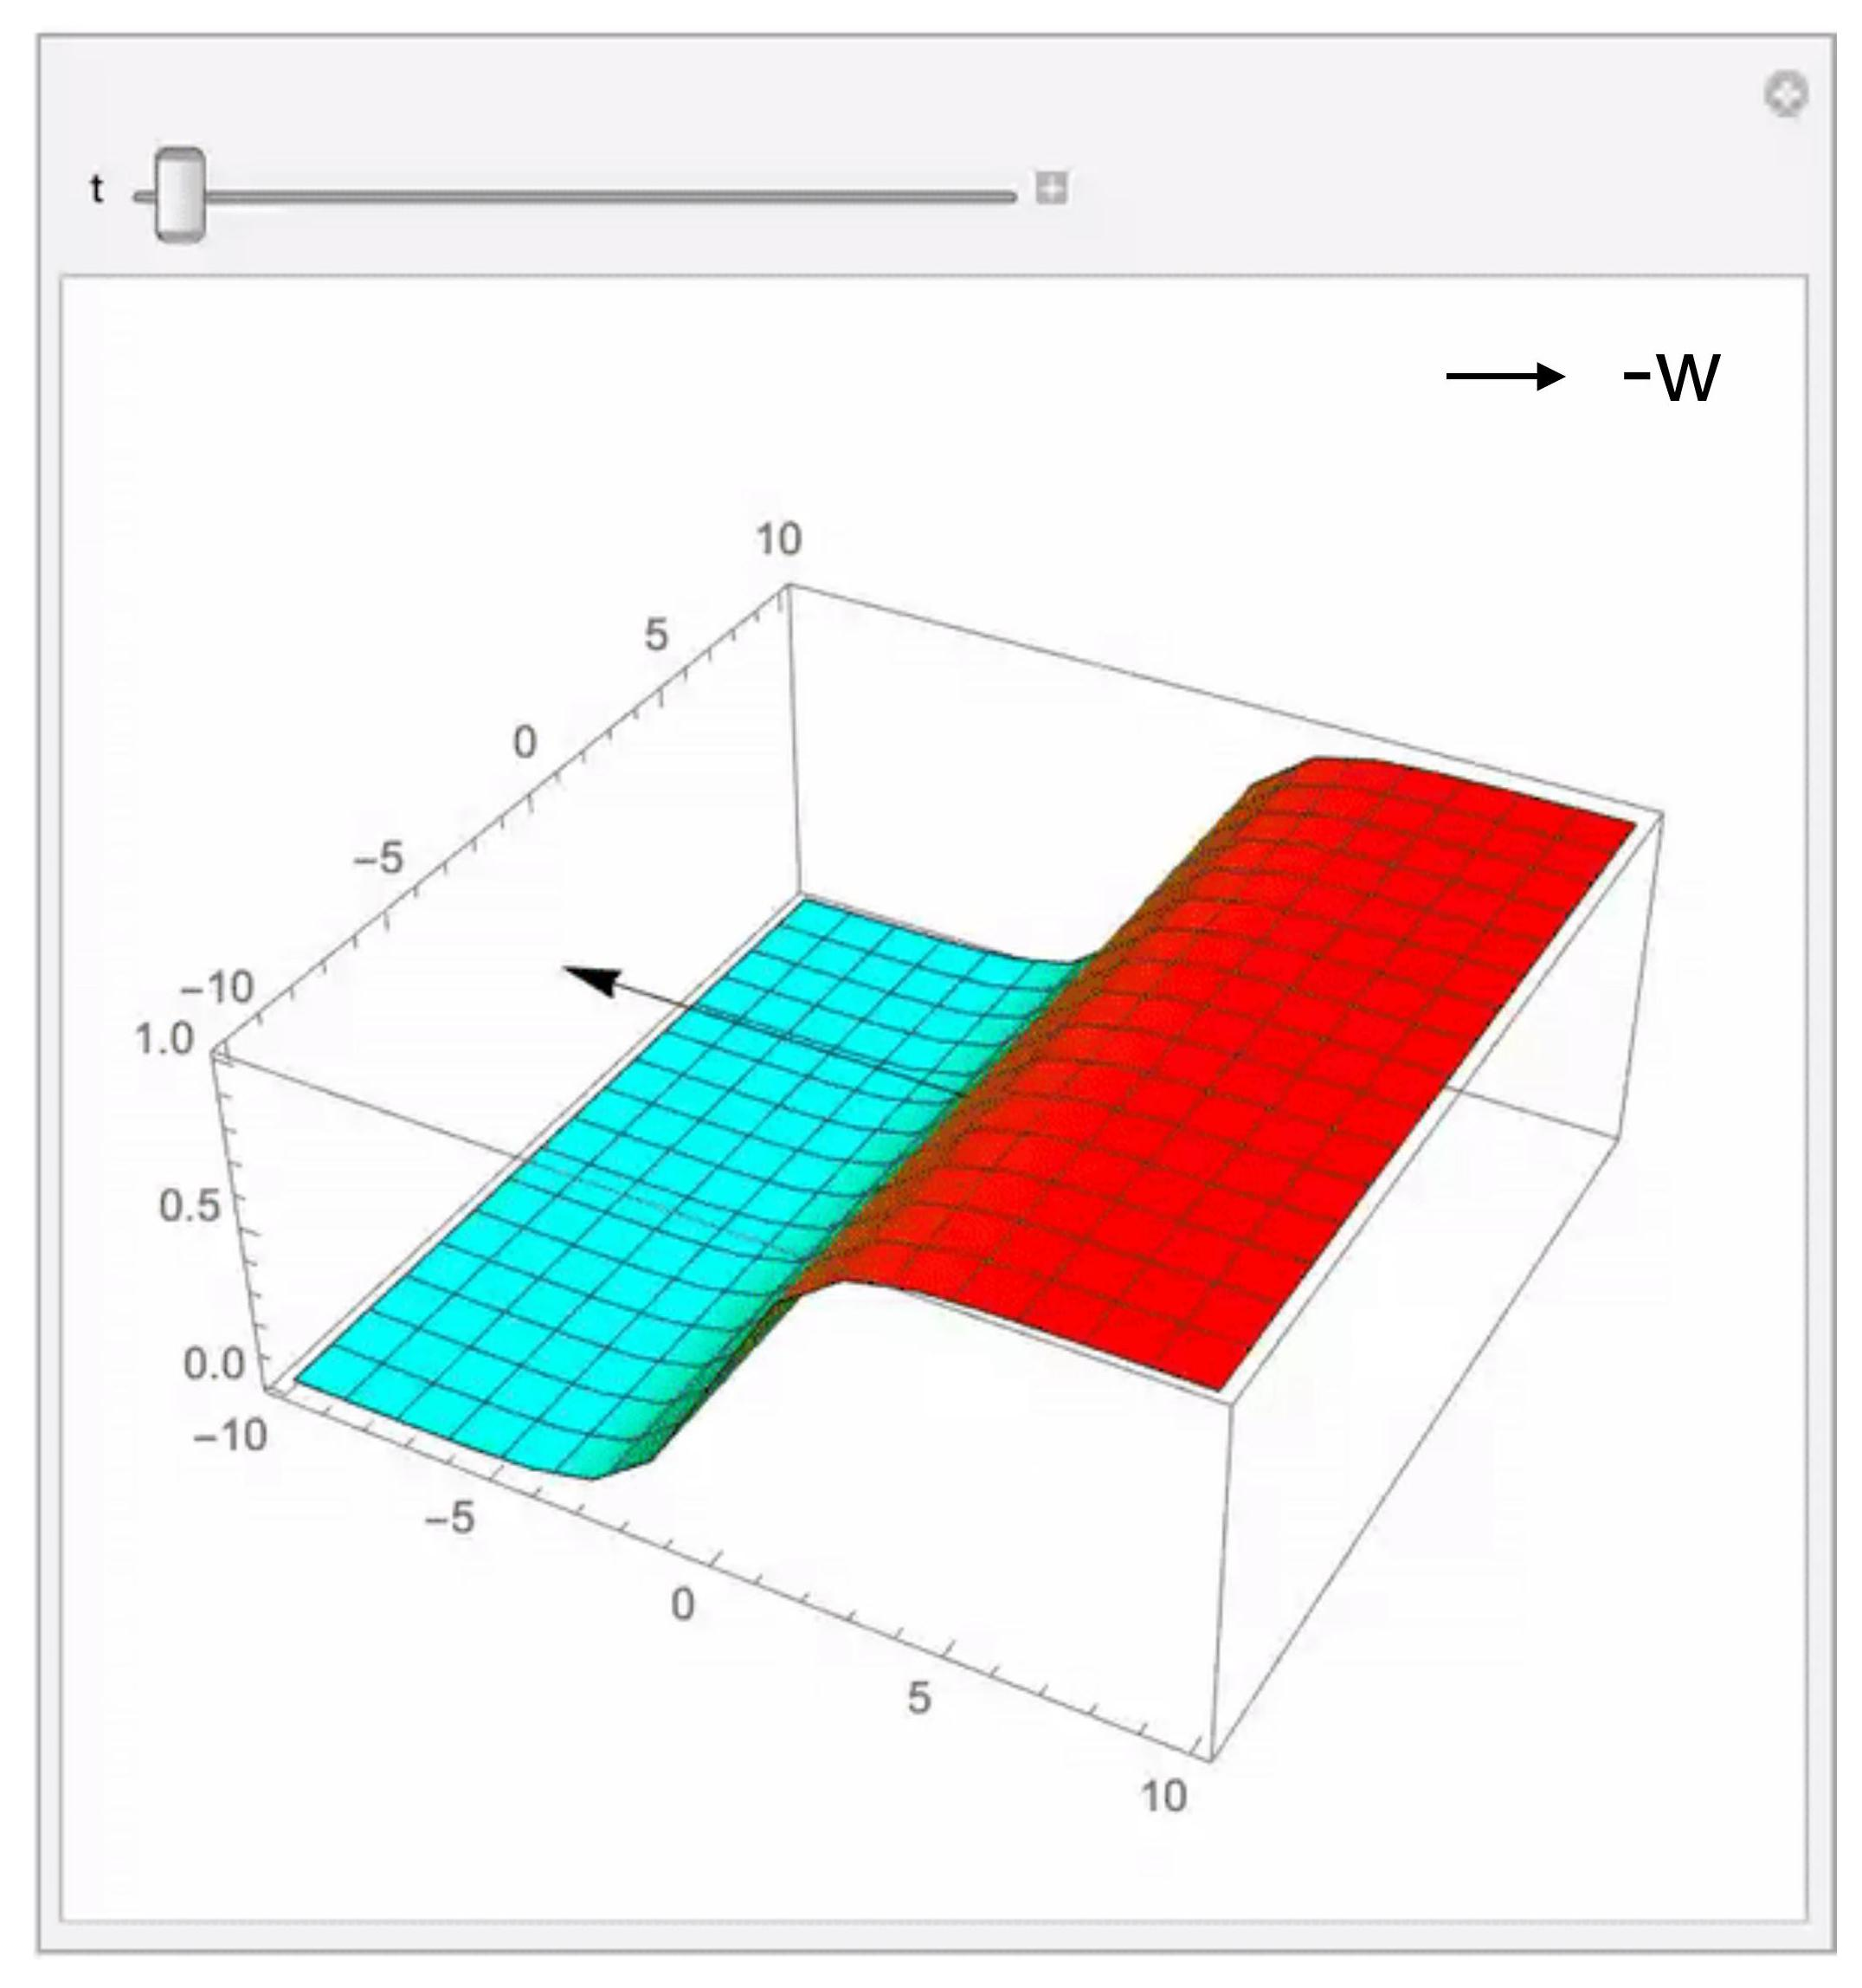
\includegraphics[max width=\textwidth]{2023_12_30_261a5c67f471a6c49904g-09}
\end{center}

$$
\sigma\left(w^{\top} x\right) \text { for }\|w\|=1
$$

The transition between the two levels happens at the hyperplane $w^{\perp}=\left\{v, v^{\top} w=0\right\}$

\section*{Scaling $w$ makes the transition faster or slower}
\begin{center}
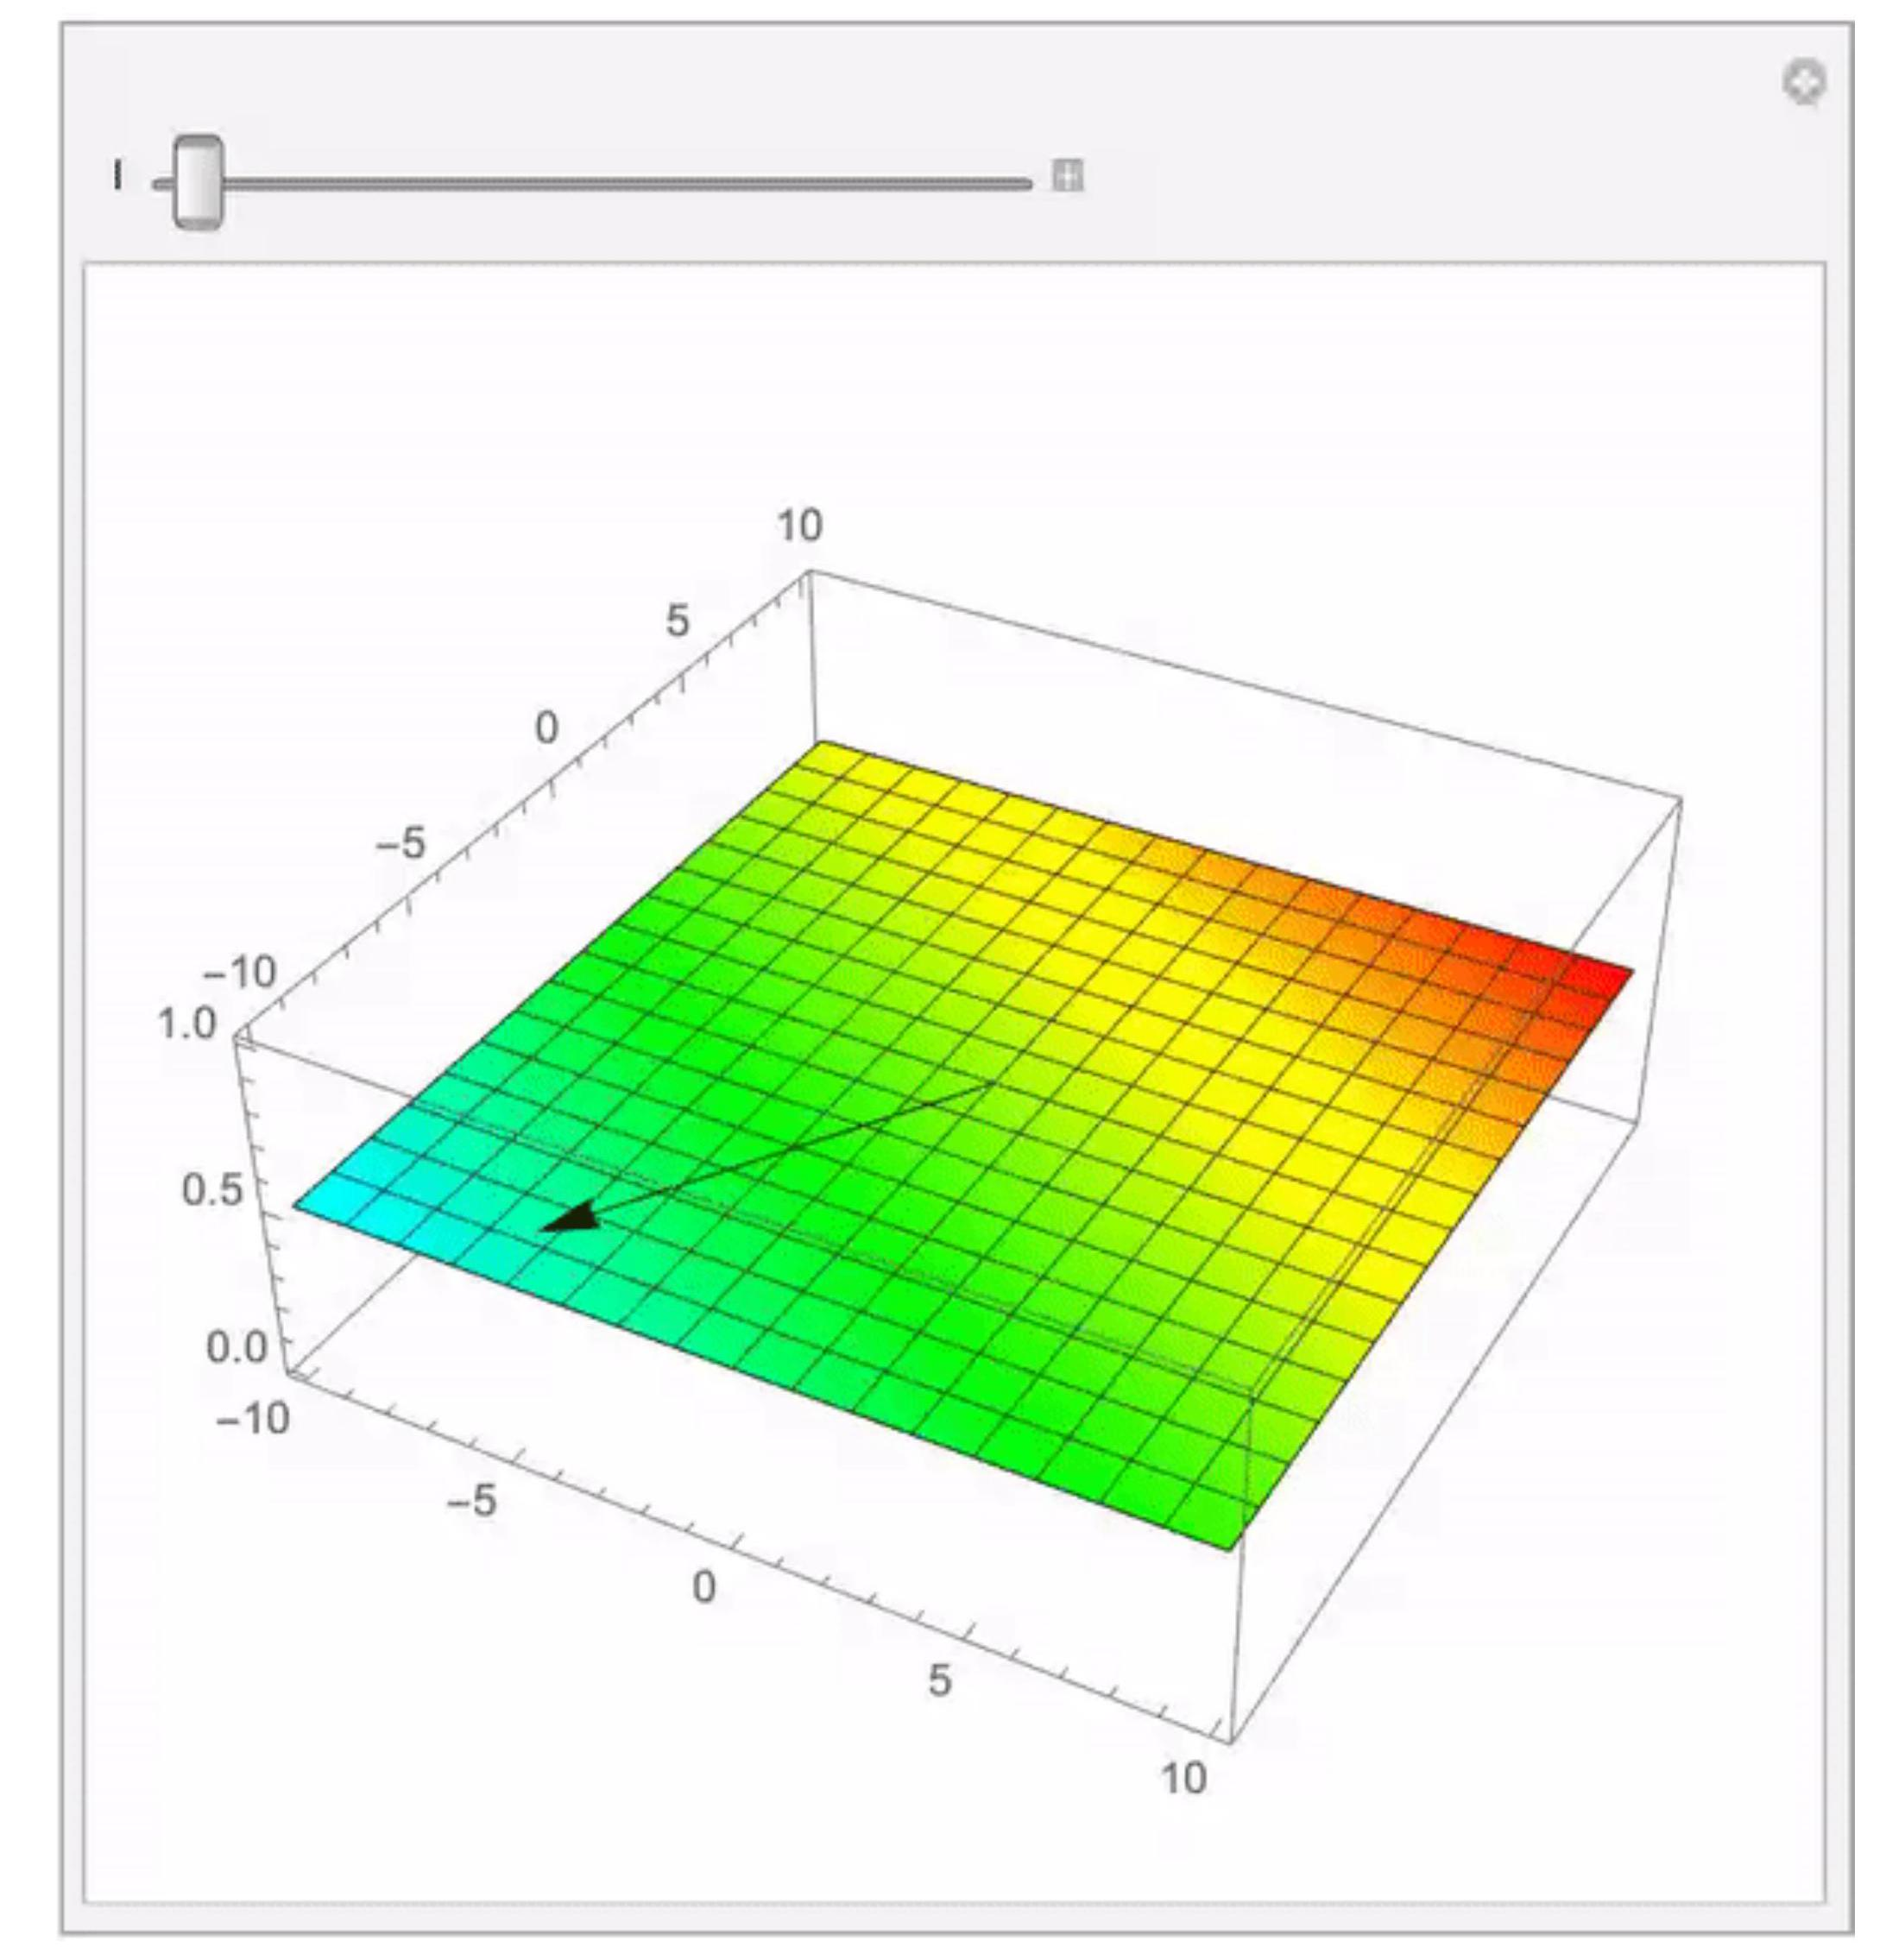
\includegraphics[max width=\textwidth]{2023_12_30_261a5c67f471a6c49904g-10(1)}
\end{center}

$\sigma\left(t \cdot w_{1}^{\top} x\right)$ for $t \in\left[e^{-10}, e^{10}\right]$

\begin{center}
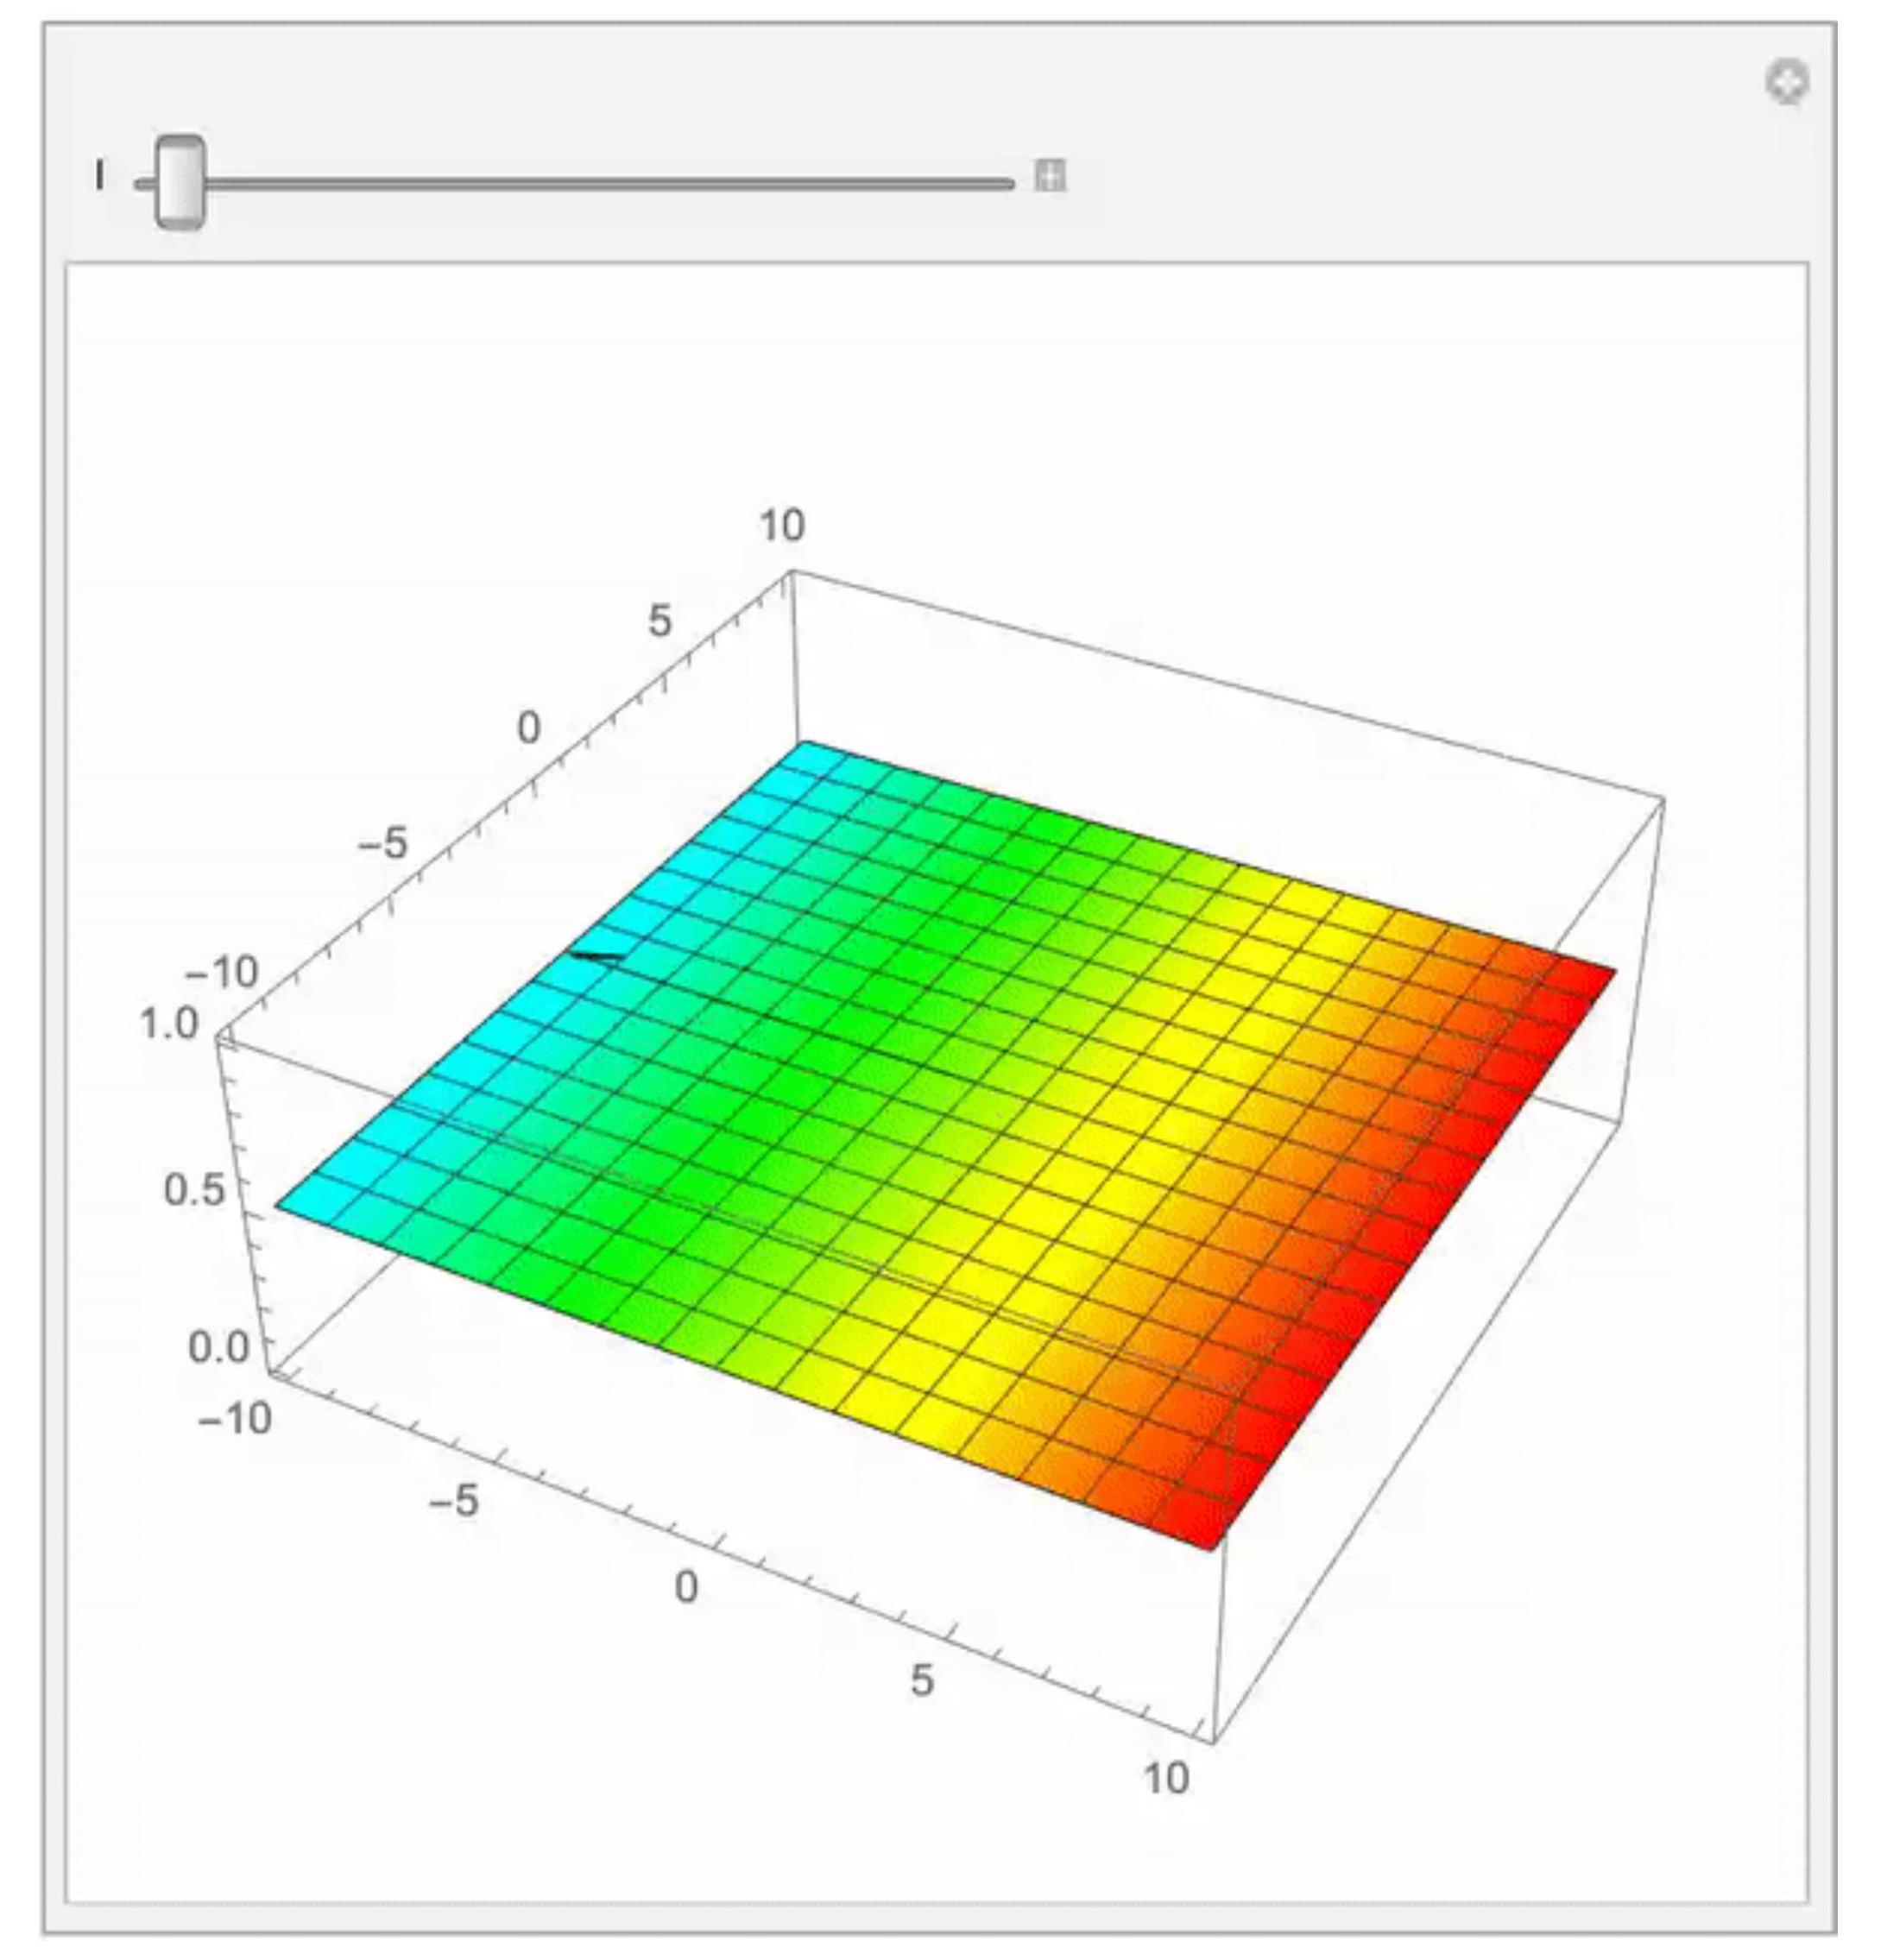
\includegraphics[max width=\textwidth]{2023_12_30_261a5c67f471a6c49904g-10}
\end{center}

$\sigma\left(t \cdot w_{2}^{\top} x\right)$ for $t \in\left[e^{-10}, e^{10}\right]$

\section*{Changing $w_{0}$ shifts the decision region along the $w$ vector}
\begin{center}
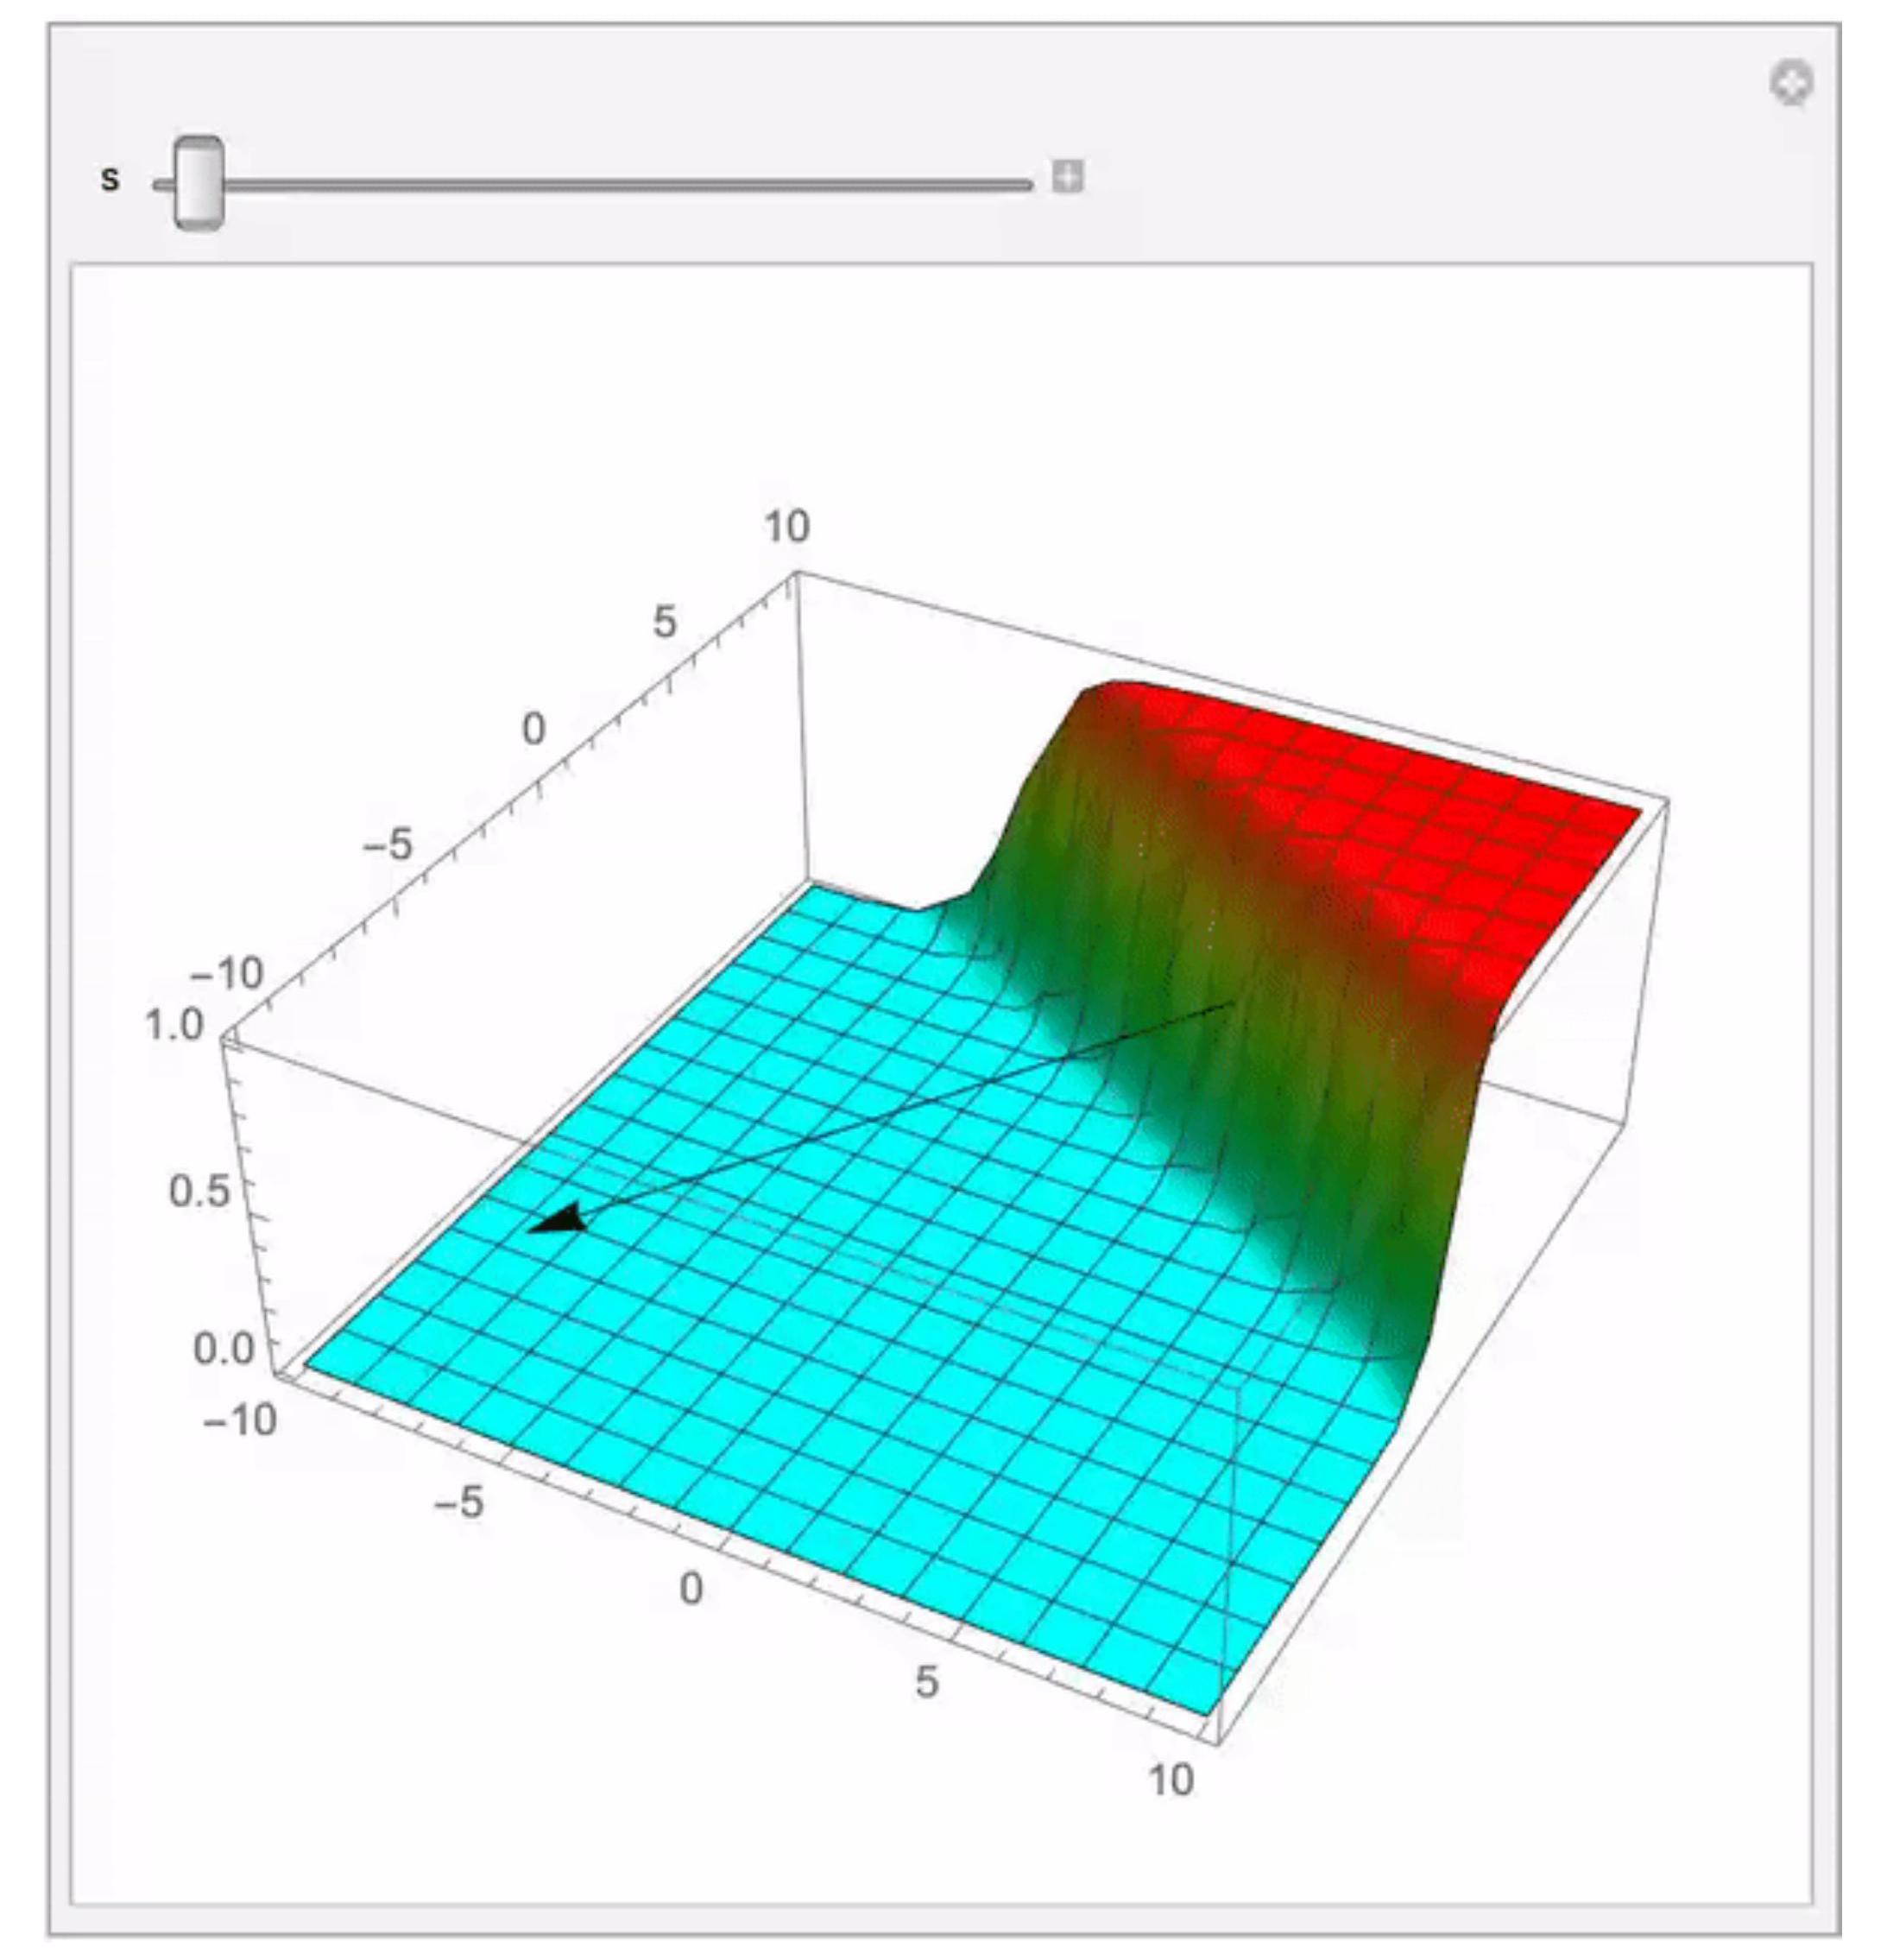
\includegraphics[max width=\textwidth]{2023_12_30_261a5c67f471a6c49904g-11(1)}
\end{center}

$$
\sigma\left(w_{1}^{\top} x+w_{0}\right) \text { for } w_{0} \in[-6,6]
$$

\begin{center}
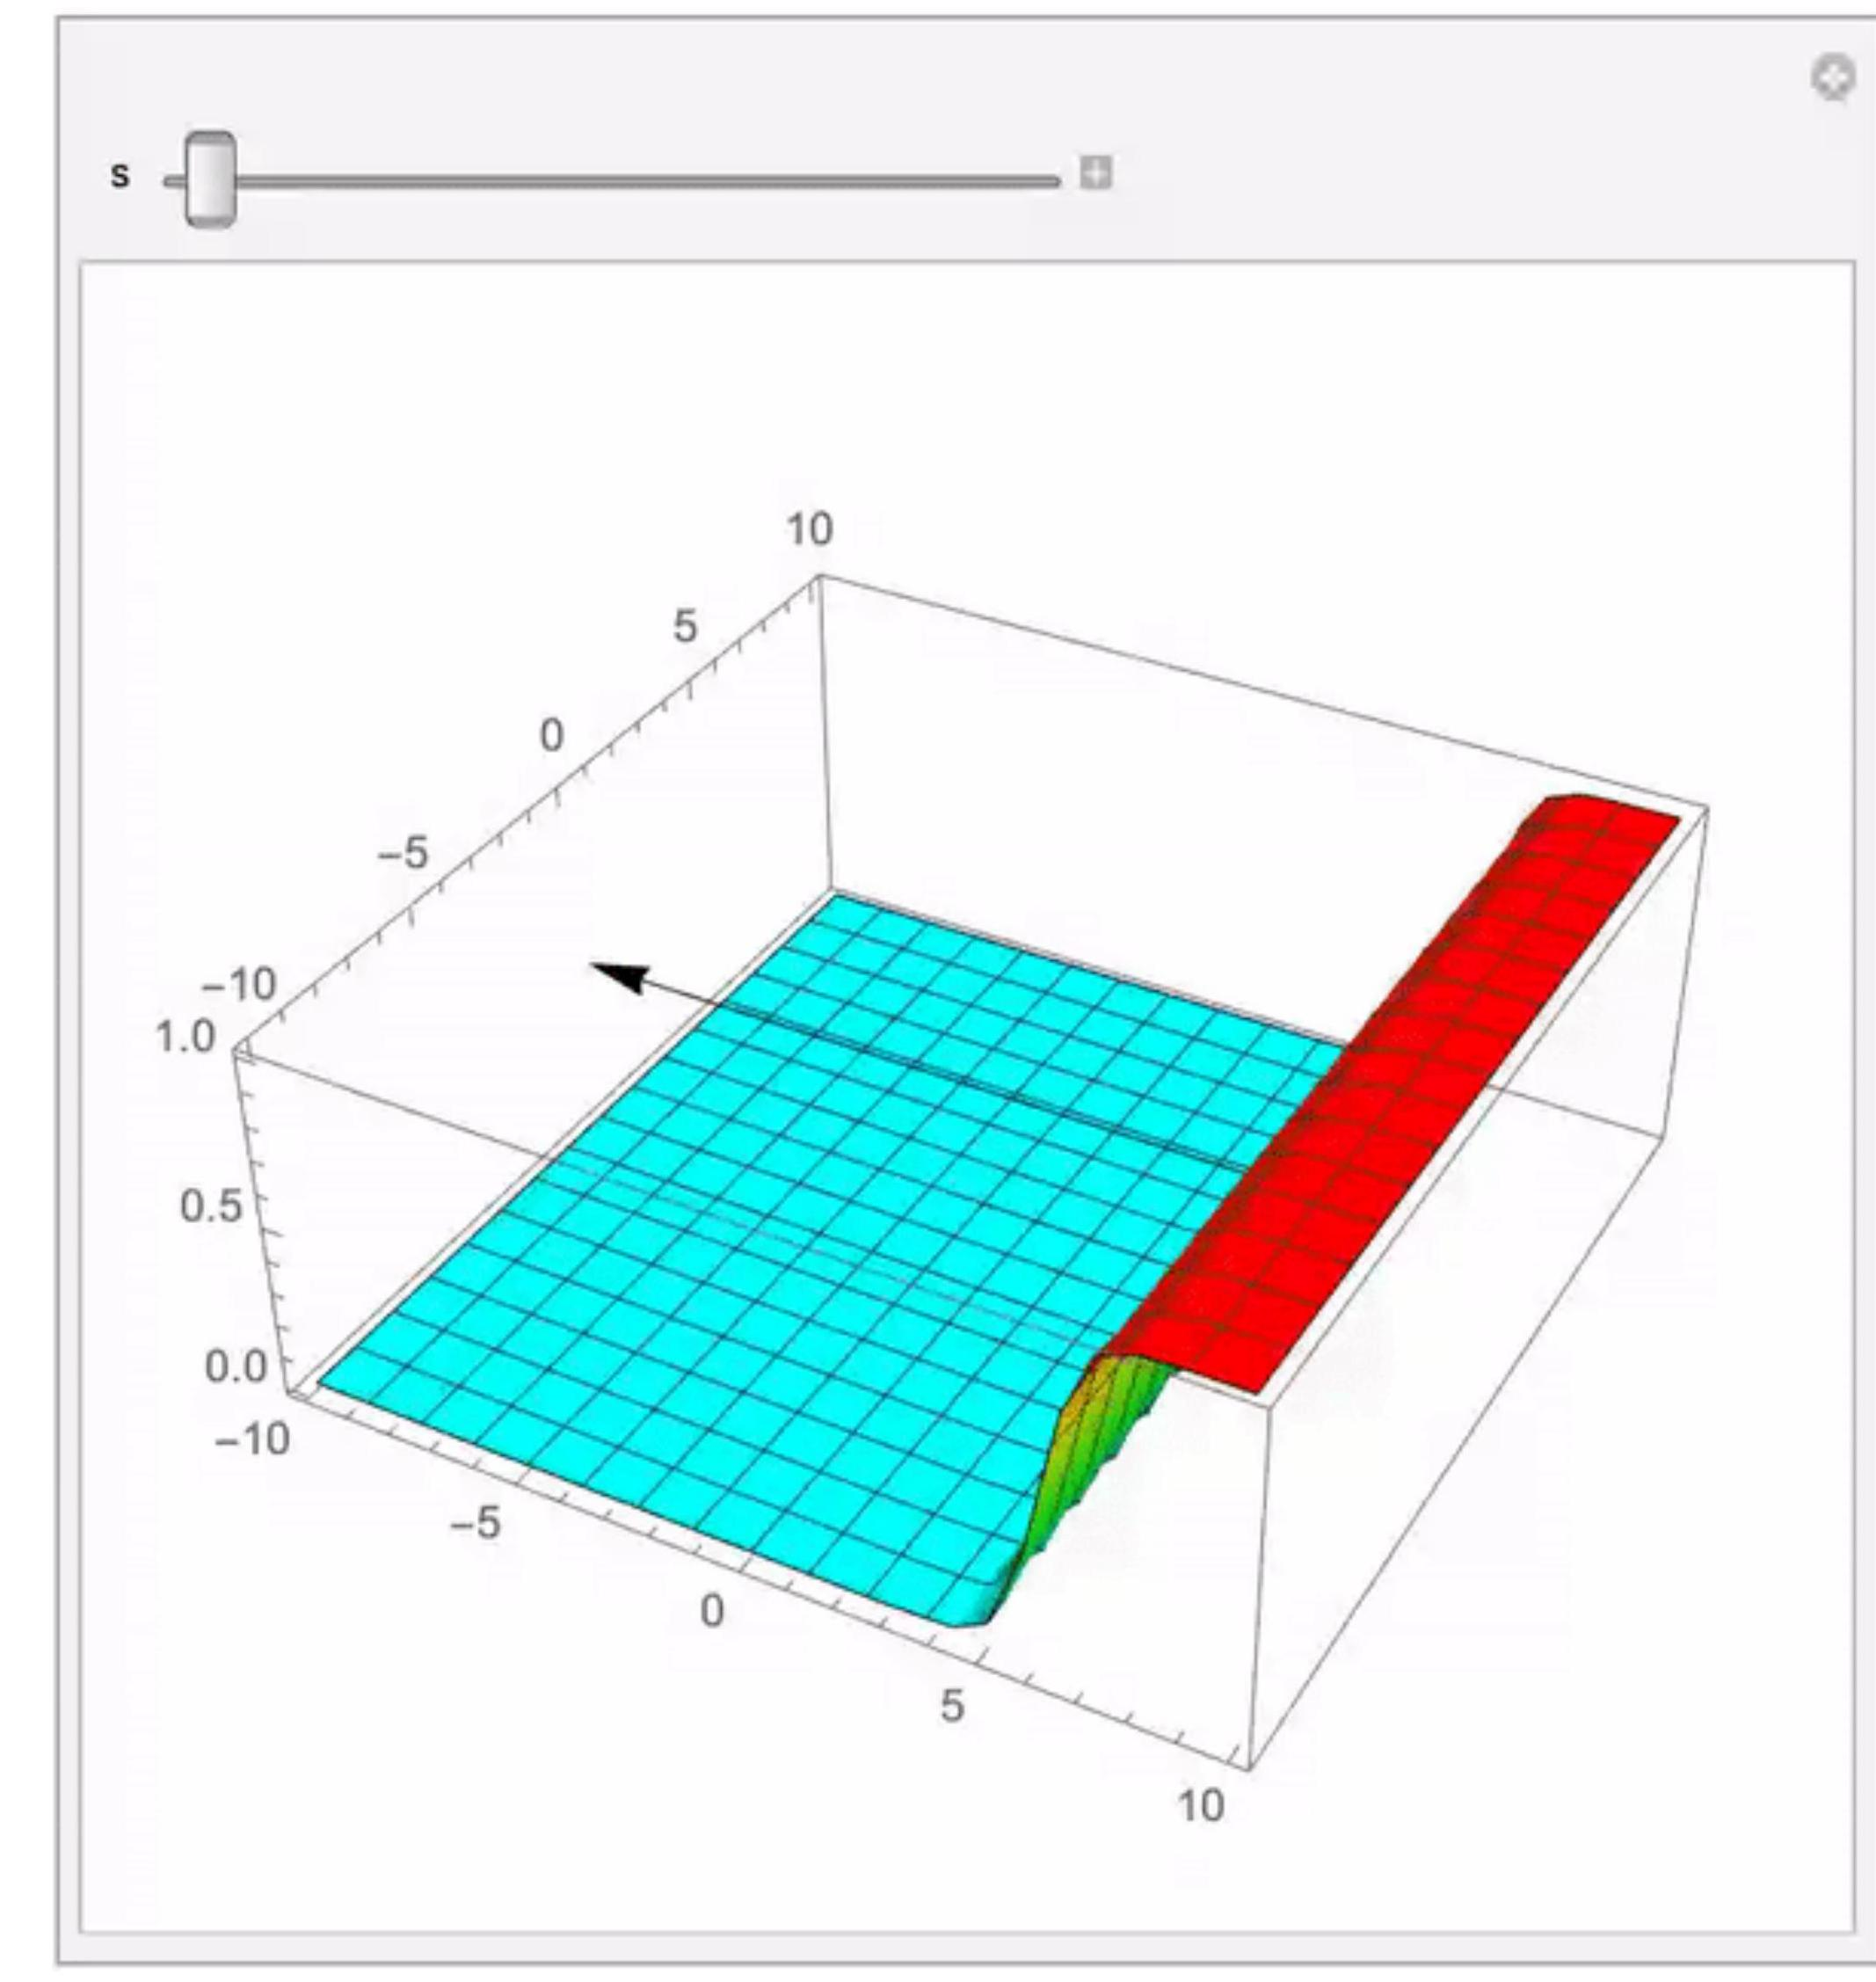
\includegraphics[max width=\textwidth]{2023_12_30_261a5c67f471a6c49904g-11}
\end{center}

$\sigma\left(w_{2}^{\top} x+w_{0}\right)$ for $w_{0} \in[-6,6]$

The transition happens at the hyperplane $\left\{v, v^{\top} w+w_{0}=0\right\}$

\section*{What about the bias term?}
We should consider a shift $w_{0}$ as there is no reason for the transition hyperplane to pass through the origin:

$$
p(1 \mid x)=\sigma\left(w^{\top} x+w_{0}\right)
$$

However, for simplicity, we will prefer to add the constant 1 to the feature vector

$$
x=\left(\begin{array}{c}
x \\
1
\end{array}\right)
$$

It is crucial for allowing to shift the decision region

Note that both options are equivalent

\section*{Maximum likelihood estimation (MLE) is a method of estimating the parameters of a statistical model}
Given i.i.d. samples $\left(z_{1}, \cdots, z_{N}\right) \sim p\left(z_{1}, \cdots, z_{N} \mid w\right)$, the MLE finds the parameters $w_{*}$ under which the observations $z_{1}, \cdots, z_{N}$ are the most likely:

$$
w_{*}=\underset{\text { Likelihood function }}{\arg \max } \underset{\nearrow}{\mathscr{L}}(w):=p\left(z_{1}, \cdots, z_{N} \mid w\right)=\prod_{\substack{\text { i.i.d. obs }}}^{N} p\left(z_{n} \mid w\right)
$$

Often more convenient to work with the negative log-likelihood:

$$
w_{*}=\arg \min [-\log (\mathscr{L}(w))]=\arg \min \sum_{n=1}^{N}-\log \left(p\left(z_{n} \mid w\right)\right)
$$

This estimator is consistent*: if the data are generated according to the model, the MLE converges to the true parameter when $n \rightarrow \infty$ In practice, data are not generated according to it, but it still provides a theoretical justification

\section*{MLE for logistic regression}
Assumption: The inputs $\mathbf{X}$ do not depend on the parameter $w$ we choose:

$$
\begin{aligned}
& \mathscr{L}(w)=p(\mathbf{y}, \mathbf{X} \mid w)=p(\mathbf{X} \mid w) p(\mathbf{y} \mid \mathbf{X}, w) \underset{\mathbf{X} \Perp w}{=} p(\mathbf{X}) p(\mathbf{y} \mid \mathbf{X}, w) \\
& \begin{aligned}
p(\mathbf{y} \mid \mathbf{X}, w) & =\Pi_{n=1}^{N} p\left(y_{n} \mid x_{n}, w\right) \\
& =\Pi_{n: y_{n}=1} p\left(y_{n}=1 \mid x_{n}, w\right) \Pi_{n: y_{n}=0} p\left(y_{n}=0 \mid x_{n}, w\right) \\
& =\Pi_{n=1}^{N} \sigma\left(x_{n}^{\top} w\right)^{y_{n}}\left[1-\sigma\left(x_{n}^{\top} w\right)\right]^{1-y_{n}}
\end{aligned}
\end{aligned}
$$

The likelihood is proportional to:

$$
\left.\mathscr{L}(w) \propto \prod_{n=1}^{N} \sigma\left(x_{n}^{\top} w\right)^{y_{n}[1}-\sigma\left(x_{n}^{\top} w\right)\right]^{1-y_{n}}
$$

\section*{Minimum of the negative log likelihood}
It is more convenient to work with the negative log-likelihood:

$$
\begin{aligned}
& -\log (p(\mathbf{y} \mid \mathbf{X}, w))=-\log \left(\prod_{n=1}^{N} \sigma\left(x_{n}^{\top} w\right)^{y_{n}}\left[1-\sigma\left(x_{n}^{\top} w\right)\right]^{1-y_{n}}\right) \\
& =-\sum_{n=1}^{N} y_{n} \log \sigma\left(x_{n}^{\top} w\right)+\left(1-y_{n}\right) \log \left(1-\sigma\left(x_{n}^{\top} w\right)\right) \\
& =\sum_{n=1}^{N} y_{n} \log \left(\frac{1-\sigma\left(x_{n}^{\top} w\right)}{\sigma\left(x_{n}^{\top} w\right)}\right)-\log \left(1-\sigma\left(x_{n}^{\top} w\right)\right) \\
& =\sum_{n=1}^{N}-y_{n} x_{n}^{\top} w+\log \left(1+e^{x_{n}^{\top} w}\right) \longleftarrow 1-\sigma(\eta)=\frac{1}{1+e^{\eta}} \Longrightarrow \frac{1-\sigma(\eta)}{\sigma(\eta)}=e^{-\eta}
\end{aligned}
$$

We obtain the following cost function we will minimize to learn the parameter $w_{*}$

$$
w_{*}=\arg \min L(w):=\frac{1}{N} \sum_{n=1}^{N}-y_{n} x_{n}^{\top} w+\log \left(1+e^{x_{n}^{\top} w}\right)
$$

*If we are considering $y \in\{-1,1\}$, we will have a different function

${ }^{\star \star}$ minimizing $\mathrm{L}$ is exactly equivalent to maximize the likelihood $\mathscr{L}$ since $p(X) \Perp w$

\section*{A side note on logistic loss}
In logistic regression, the negative log likelihood is equivalent to ERM for the logistic loss (a surrogate for $0-1$ loss, as discussed yesterday)

\begin{itemize}
  \item Logistic loss for $y \in\{0,1\}$ :
\end{itemize}

$$
\ell(y, g(x))=-y g(x)+\log (1+\exp (g(x)))
$$

\begin{itemize}
  \item Logistic loss for $y \in\{-1,1\}$ :
\end{itemize}

$$
\ell(y, g(x))=\log (1+\exp (-y g(x)))
$$

Note: the logistic loss can be applied in modern machine learning as well: $g(x)$ can represent the output of a neural network

\section*{Gradient of the negative log likelihood}
To minimize L, let's first look at its stationary points by computing its gradient:

$\nabla L(w)=\nabla\left[\frac{1}{N} \sum_{n=1}^{N} \log \left(1+e^{x_{n}^{\top} w}\right)-y_{n} x_{n}^{\top} w\right]=\frac{1}{N} \sum_{n=1}^{N} \frac{e^{x_{n}^{\top} w} x_{n}}{1+e^{x_{n}^{\top} w}}-y_{n} x_{n}=\frac{1}{N} \sum_{n=1}^{N}\left(\sigma\left(x_{n}^{\top} w\right)-y_{n}\right) x_{n}$

Which can be written under the matrix form $\mathbf{x}=\left[\begin{array}{c}x_{1}^{\top} \\ \vdots \\ x_{n}^{\top}\end{array}\right] \in \mathbb{R}^{n \times d}$ and $\mathbf{y}=\left[\begin{array}{c}y_{1} \\ \vdots \\ y_{n}\end{array}\right] \in \mathbb{R}^{n}$

$$
\nabla L(w)=\frac{1}{N} \mathbf{X}^{\top}(\sigma(\mathbf{X} w)-\mathbf{y})
$$

\begin{itemize}
  \item Same gradient as in LS but with $\sigma$
  \item No closed form solution to $\nabla L(w)=0$
  \item Good news: the cost function $L$ is convex
\end{itemize}

\section*{Convexity of the loss function $L$}
Claim: The function

$$
L(w)=\frac{1}{N} \sum_{n=1}^{N}-y_{n} x_{n}^{\top} w+\log \left(1+e^{x_{n}^{\top} w}\right)
$$

is convex in the weight vector $w$

Proof: $L$ is obtained through simple convexity preserving operations:

\begin{enumerate}
  \item Positive combinations of convex functions is convex

  \item Composition of a convex and a linear functions is convex

  \item A linear function is both convex and concave

  \item $\eta \mapsto \log \left(1+e^{\eta}\right)$ is convex

\end{enumerate}

\section*{Convexity of the loss function $L$}
Claim: The function

$$
L(w)=\frac{1}{N} \sum_{n=1}^{N}-y_{n} x_{n}^{\top} w+\log \left(1+e^{x_{n}^{\top} w}\right)
$$

is convex in the weight vector $w$

Proof: $L$ is obtained through simple convexity preserving operations:

\begin{enumerate}
  \item Positive combinations of convex f Proof of 4: $h(\eta):=\log \left(1+e^{\eta}\right)$ is cvx

  \item Composition of a convex and a lir

  \item A linear function is both convex ar

\end{enumerate}

$h^{\prime}(\eta)=\frac{e^{\eta}}{1+e^{\eta}}=\sigma(\eta)$
4. $\eta \mapsto \log \left(1+e^{\eta}\right)$ is convex

$$
h^{\prime \prime}(\eta)=\sigma^{\prime}(\eta)=\frac{e^{\eta}}{\left(1+e^{\eta}\right)^{2}} \geq 0
$$

\section*{Proof of the convexity of $L$}
\begin{enumerate}
  \setcounter{enumi}{1}
  \item Composition of a convex and a linear functions is convex
  \item $\eta \mapsto \log \left(1+e^{\eta}\right)$ is convex
\end{enumerate}

$$
\log \left(1+e^{x_{n}^{\top} w}\right) \text { is convex }
$$

\begin{enumerate}
  \setcounter{enumi}{2}
  \item A linear function is both convex and concave
\end{enumerate}

$$
-y_{n} x_{n}^{\top} w \text { is convex }
$$

\begin{enumerate}
  \item Positive combinations of convex functions is convex
\end{enumerate}

$$
L(w)=\frac{1}{N} \sum_{n=1}^{N}-y_{n} x_{n}^{\top} w+\log \left(1+e^{x_{n}^{\top} w}\right) \text { is convex }
$$

\section*{Second proof: Hessian of $L$ is psd}
The Hessian $\nabla^{2} L$ is the matrix whose entries are the second derivatives $\frac{\partial^{2}}{\partial w_{i} \partial w_{j}} L(w)$

$$
\begin{aligned}
\nabla^{2} L(w) & =\nabla[\nabla L(w)]^{\top} \\
& =\nabla\left[\frac{1}{N} \sum_{n=1}^{N} x_{n}\left(\sigma\left(x_{n}^{\top} w\right)-y_{n}\right)\right]^{\top} \\
& =\frac{1}{N} \sum_{n=1}^{N} \nabla \sigma\left(x_{n}^{\top} w\right) x_{n}^{\top}=\frac{1}{N} \sum_{n=1}^{N} \sigma\left(x_{n}^{\top} w\right)\left(1-\sigma\left(x_{n}^{\top} w\right)\right) x_{n} x_{n}^{\top}
\end{aligned}
$$

It can be written under the matrix form:

$$
\nabla^{2} L(w)=\frac{1}{N} \mathbf{X}^{\top} S \mathbf{X}, \quad \text { where } S=\operatorname{diag}\left[\sigma\left(x_{n}^{\top} w\right)\left(1-\sigma\left(x_{n}^{\top} w\right)\right)\right] \succcurlyeq 0
$$

$\Rightarrow \mathrm{L}$ is convex since $\nabla^{2} L(w) \geqslant 0$

\section*{How to minimize the convex function L?}
Gradient descent:

$$
\left\{\begin{array}{l}
w_{0} \in \mathbb{R}^{d} \\
w_{t+1}=w_{t}-\frac{\gamma_{t}}{N} \sum_{n=1}^{N}\left(\sigma\left(x_{n}^{\top} w_{t}\right)-y_{n}\right) x_{n}
\end{array}\right.
$$

can be slow

Stochastic gradient descent

$$
\left\{\begin{array}{l}
w_{0} \in \mathbb{R}^{d} \\
w_{t+1}=w_{t}-\gamma_{t}\left(\sigma\left(x_{n_{t}}^{\top} w_{t}\right)-y_{n_{t}}\right) x_{n_{t}}
\end{array} \text { where } \mathbb{P}\left[n_{t}=n\right]=1 / N\right.
$$

is faster but converges slower

\section*{Newton's method uses second order information}
Newton's method minimizes the quadratic approximation:

$$
\begin{gathered}
L(w) \sim L\left(w_{t}\right)+\nabla L\left(w_{t}\right)^{\top}\left(w-w_{t}\right)+\frac{1}{2}\left(w-w_{t}\right)^{\top} \nabla^{2} L\left(w_{t}\right)\left(w-w_{t}\right):=\phi_{t}(w) \\
\tilde{w}=\arg \min \phi_{t}(w) \Longrightarrow \nabla L\left(w_{t}\right)+\nabla^{2} L\left(w_{t}\right)\left(\tilde{w}-w_{t}\right)=0
\end{gathered}
$$

Newton's method: $\quad w_{t+1}=w_{t}-\gamma_{t} \nabla^{2} L\left(w_{t}\right)^{-1} \nabla L\left(w_{t}\right)$

The step-size is needed to ensure convergence (damped Newton's method)

The convergence is typically faster than with gradient descent but the computational complexity is higher (computing Hessian and solving a linear system)

\section*{Problem when the data are linearly separable}
$$
\inf _{w} L(w)=0=\lim _{\alpha \rightarrow \infty} L(\alpha \cdot \bar{w})
$$

The inf value is not attained for a finite $w$

If we use an optimization algorithm, the weights will go to $\infty$

Solution: add a $\ell_{2}$-regularization

\begin{itemize}
  \item ridge logistic regression:
\end{itemize}

$\frac{1}{N} \sum_{n=1}^{N}-y_{n} x_{n}^{\top} w+\log \left(1+e^{x_{n}^{\top} w}\right)+\frac{\lambda}{2}\|w\|_{2}^{2}$

\begin{center}
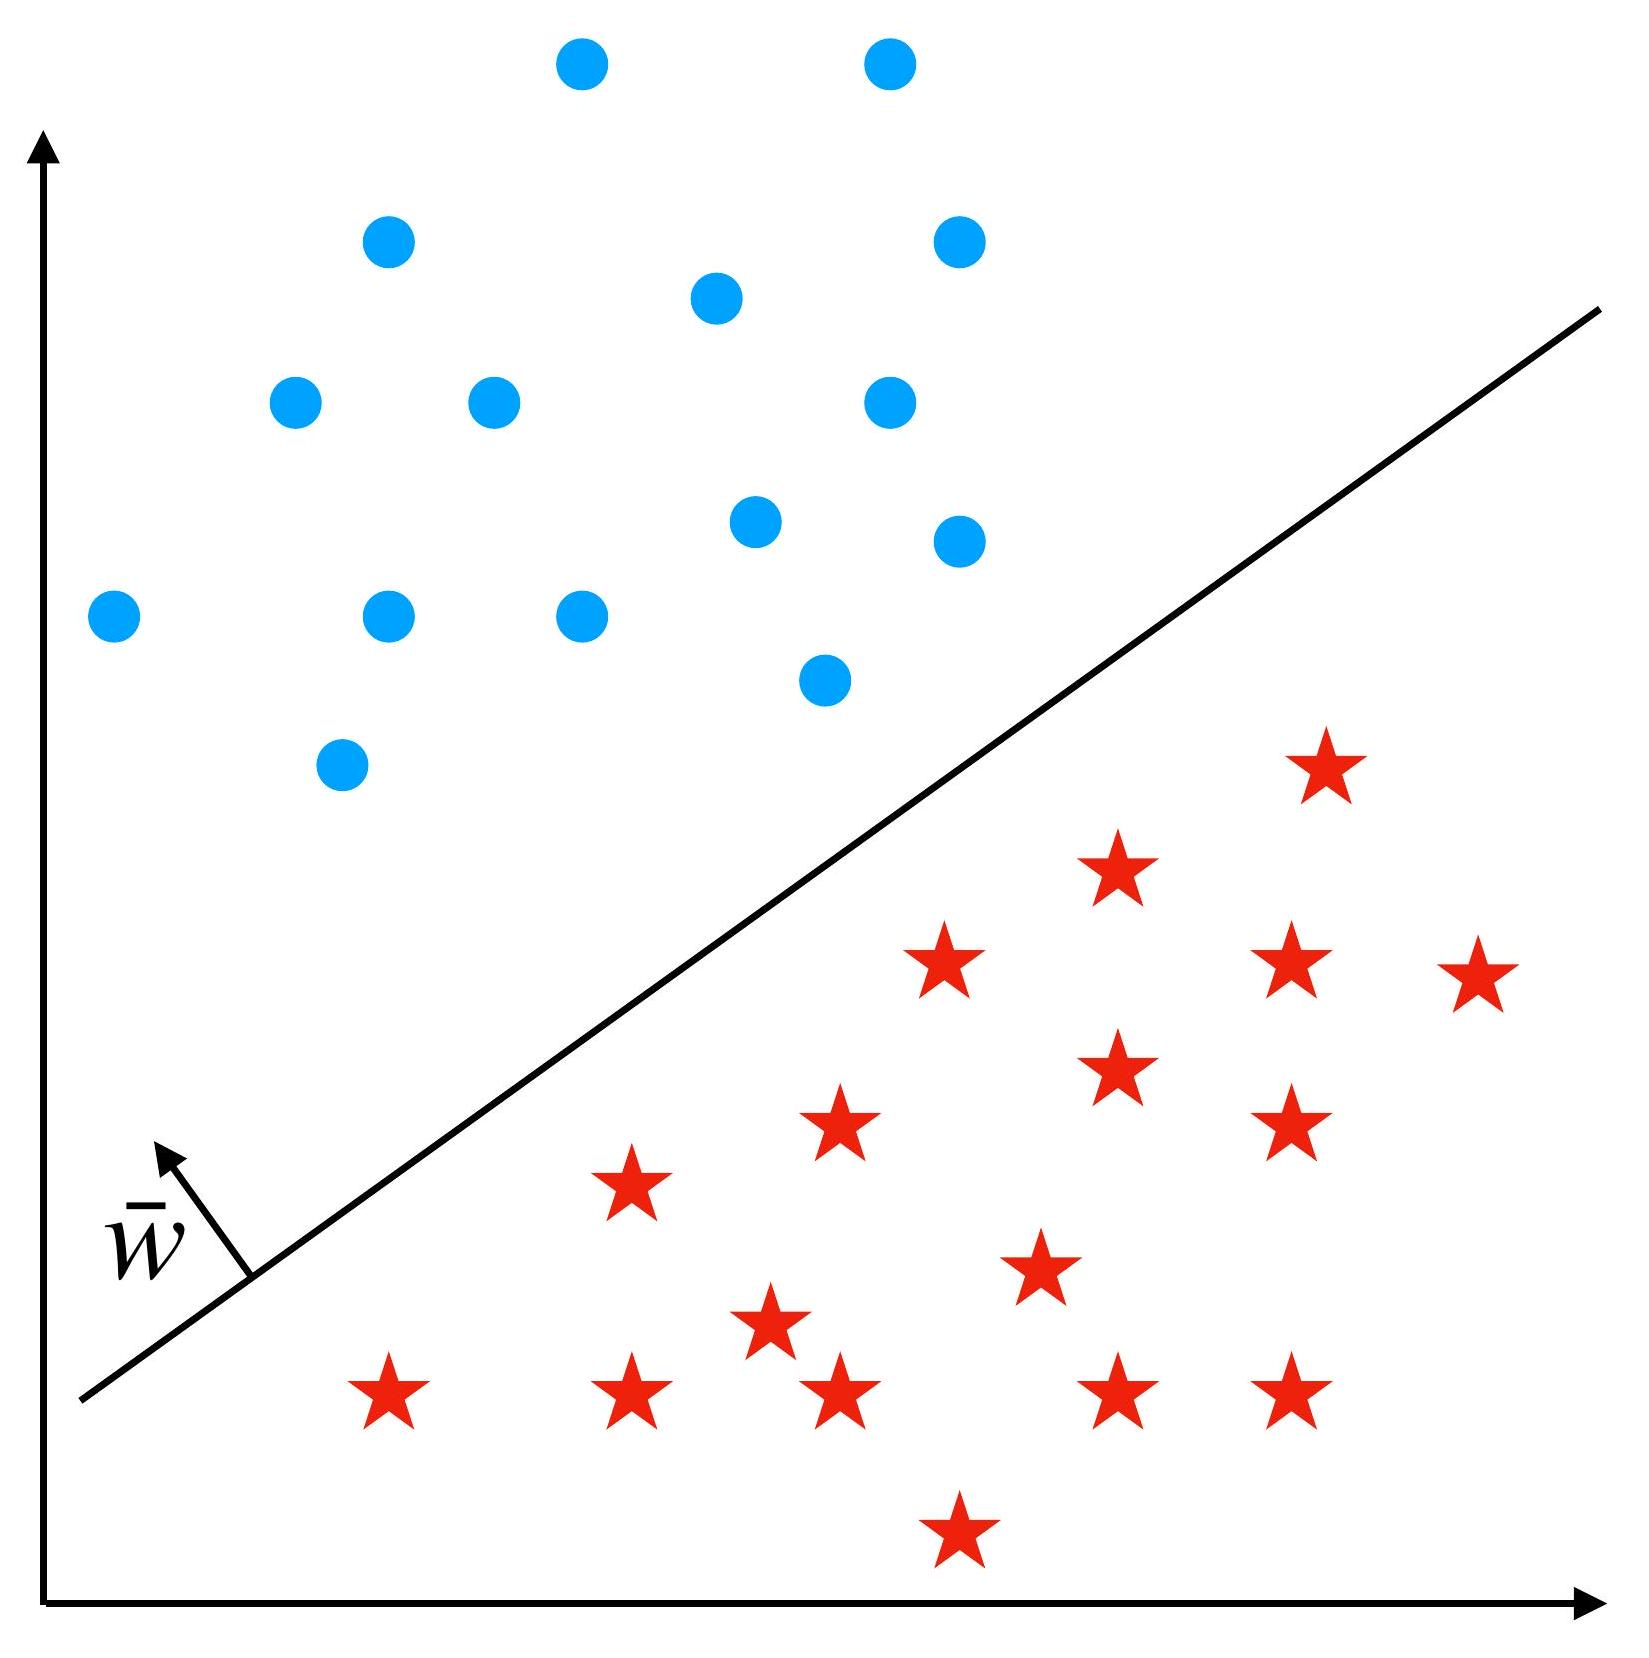
\includegraphics[max width=\textwidth]{2023_12_30_261a5c67f471a6c49904g-24}
\end{center}

\begin{itemize}
  \item Optimization perspective: stabilize the optimization process
\end{itemize}

$L(w)=\frac{1}{N} \sum_{n=1}^{N}-y_{n} x_{n}^{\top} w+\log \left(1+e^{x_{n}^{\top} w}\right)$

\begin{itemize}
  \item Statistical perspective: avoid overfitting
\end{itemize}

\section*{Recap}
\begin{itemize}
  \item Logistic regression:

  \item Maps inputs to output class probabilities

  \item Exhibits robustness towards unbalanced data and extreme values

  \item How to solve logistic regression?

  \item By minimizing the negative log-likelihood (a.k.a. logistic loss)

  \item Using gradient methods or second-order methods

  \item Not ideal when data is linearly separable?

  \item Weights go to infinity

  \item A solution is to add a penalty term, e.g. $\ell_{2}$-regularization

\end{itemize}

\end{document}